\documentclass[12 pt,a4 paper ]{scrreprt}
 
\usepackage[utf8]{inputenc}
\usepackage[naustrian]{babel}
\usepackage{lmodern}
\usepackage[T1]{fontenc}
\usepackage{graphicx}
\usepackage{amsmath}
\usepackage{float}
\usepackage{amsmath,amssymb,amstext}
%\usepackage{pgfplots}

\usepackage[headsepline,plainheadsepline]{scrpage2}
\pagestyle{scrheadings}
\ihead[\rightmark]{\rightmark} \chead[]{}
%\ohead[\pagemark]{\pagemark} \cfoot[]{}

\automark{chapter}
\renewcommand{\chaptermark}[1]{\markright{\ #1}}










\begin{document}

\tableofcontents	
	
	
	
	
	
\chapter{Auswertung der Versuche}

\section{Allgemeines}

In diesem Kapitel werden die Unterschiede zwischen den 4 Versuchen erläutert und die Ergebnisse, sowie das Versagen der einzelnen Versuche erklärt. Weiters werden allgemeine Anmerkung zu dem Versuchen beschrieben. Die Tabelle \ref{tab:Versuchsprogramm}  soll einen Überblick über die Großbauteilversuche bzw. über die Unterschiede der einzelnen Versuche geben.

\begin{table}[h]
\caption{Versuchsprogramm}
\begin{center}
\begin{tabular}{|c|c|c|c|c|c|}
\hline 
\multicolumn{6}{|c|}{ Übersicht} \\ 
\hline 
Versuch & Abmessungen  & Schraubenanzahl & Kleber & Belastung & Aushärtezeit \\ 

&  l x b x h in [m] & (Fa. SFS) & (FA. Sika) & (kN/min] & Tage \\ 
\hline\hline
1 & 7,40 x 0,50 x 0,33 & 28 & Sikadur 31 & 4 & 14 \\ 
\hline 
2  & 7,40 x 0,50 x 0,33 & 8 & ElastoCem 109 & 4 & 21 \\ 
\hline 
3 & 7,40 x 0,50 x 0,33 & 12 & Sikatop 107 & Kapitel 3.7 & 28 \\ 
\hline 
4  & 7,40 x 0,50 x 0,33 & - & Sikatop 107 & Kapitel 3.7 & 28 \\ 
\hline 
\end{tabular} 
\end{center}
\label{tab:Versuchsprogramm}
\end{table}

\section{1 Versuch}

\subsection{Anmerkung:}

Der Schichtenaufbau ist wie im Kapitel ..3 beschrieben. Die Anordnung der Schrauben ist aus der Abbildung \ref{1versuch} zu entnehmen. Es wurde wie in der Tabelle \ref{tab:Versuchsprogramm}  aufgelistet, der Kleber SikaDur 31-A Normal verwendet für die Probe verwendet. Die Belastungsgeschwindigkeit betrüg 4 [kN/min]. 


\begin{figure}[h]
\begin{center}
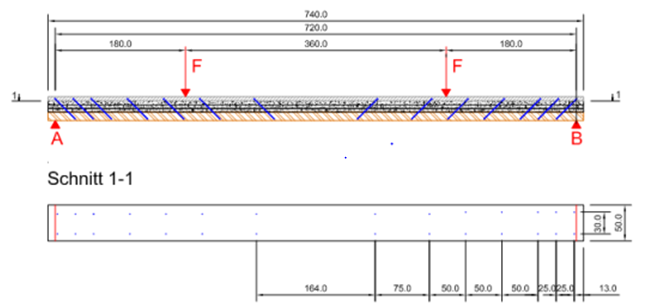
\includegraphics[scale =1.0]{1versuch.png}
\caption{Darstellung des 1 Großbauteilversuch, mit Verbindungsmittel und Lasteinleiung}
\label{1versuch}
\end{center}
\end{figure}

\subsection{Versagensbeschreibung und Auswertung}


\begin{figure}[h]
\begin{minipage}[hbt]{7cm}
	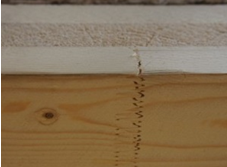
\includegraphics[width=7cm]{keilzinkung.png}
	\caption{Versagen der Keilzinkung unter der Lasteinleitung vom Auflager A }
	\label{keilzinkung}
\end{minipage}
\hfill
\begin{minipage}[hbt]{8cm}
Das erste Versagen wurde bei einer Last von 58 kN festgestellt. Unter der Last F vom Auflager A, brach die Keilzinkung der Brettsperrholzplatte. In der Abbildung \ref{keilzinkung} ist der Schaden am Bauteil darstellt.
Beim weiteren Belasten traten zunächst Risse im Beton zwischen der Kraft F und dem Auflager A auf. Die maximale Belastung betrug 78 kN. Bei dieser Last hat die Verbundfuge zwischen Holz und Holzspanbeton im Bereich zwischen dem Betonriss und dem Auflager A versagt.
\end{minipage}
\end{figure}


\begin{figure}[h]
\begin{minipage}[hbt]{7cm}
	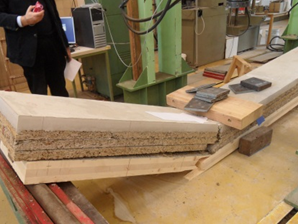
\includegraphics[width=6cm]{bruch_1versuch.png}
	\caption{Bruch nach Wiederbelastung }
	\label{1bruch}
\end{minipage}
\hfill
\begin{minipage}[hbt]{7cm}
Nach dem ersten Versagen und der Erreichung der maximalen Last, wurde der Bauteil  nochmals belastet. Durch den nicht vorhandenen Verbund ergab sich ein Lastabfall auf eine Bruchlast von 48 kN. In der Abbildung \ref{1bruch} ist die Bruchstelle nahe der Krafteinleitung dargestellt. An dieser Stelle ist auch die Keilzinkung angeordnet und der Betonriss.
\end{minipage}
\end{figure}

\begin{figure}
\begin{minipage}[hbt]{5cm}
	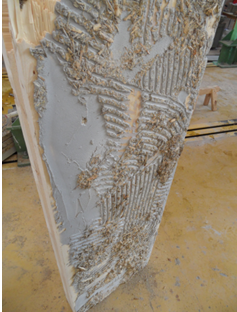
\includegraphics[width=6cm]{bruchbild.png}
	\caption{Bruchbild der CLT-Platte }
	\label{bruchbild}
\end{minipage}
\hfill
\begin{minipage}[hbt]{7cm}
Durch den Bruch konnte danach die Fuge zwischen Holzspanbeton und Holz betrachtet werden (Abbildung \ref{bruchbild}). Es zeigte sich, dass ca. ein Viertel der Fläche ungenügenden Verbund hatte. Bei näherer Betrachtung wurde ersichtlich, dass in diesem Bereich des Trägers zwei Schrauben nicht aus dem Holz aufgezogen waren, sondern gebrochen sind. Die Restlichen sechs Schrauben versagten durch Herausziehen aus der Brettsperrholzplatte. Ein Grund für das Versagen der Verbundfuge und der Keilzinkung, dürfte in der ungenügenden Vernetzung der Klebeschicht zwischen Holz und Holzspanbeton liegen. Durch den unzureichenden Verbund kam es zu höheren Biegespannungen in den Teilquerschnitten Holz und Beton und damit zum Bruch der Keilzinkung.
\end{minipage}
\end{figure}


\clearpage

\begin{figure}
\begin{center}
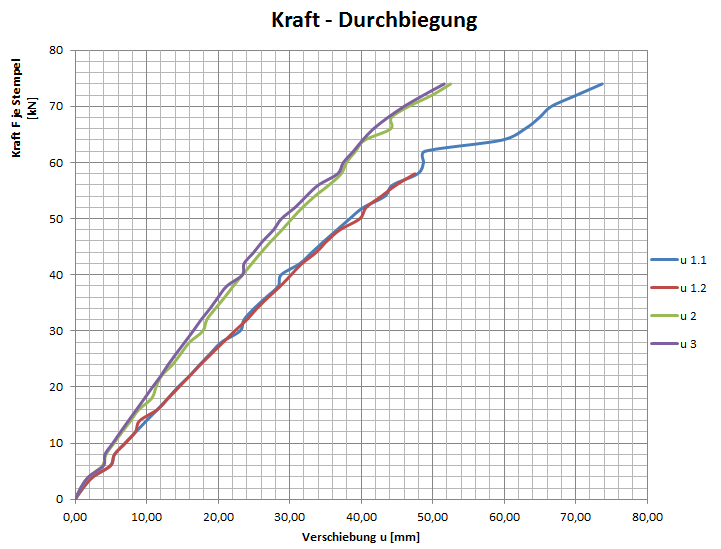
\includegraphics[scale =0.9]{1_versuch_kraft_durchbiegung.png}
\caption{1 Versuch: Kraft-Durchbiegung}
\label{1 Versuch: Kraft-Durchbiegung}
\end{center}
\end{figure}
In der Abbildung \ref{1 Versuch: Kraft-Durchbiegung} ist die Arbeitslinie der Kraft Durchbiegung dargestellt. Die angegebene Kraft bezieht sich auf einen Stempel mit der Last F. Die Verschiebungen wurden nicht in Trägermitte gemessen, sondern am Rand der Träger, damit man die Verschiebung ablesen konnte, ohne im Gefahrenbereich des Trägers zu sein. Um eine eventuelle Torsion im Versuch ausschließen zu können wurde in der Trägermitte zwei Messuhren am Rand angebracht. Die Arbeitslinie weist eine annähernd linearen Bereich bis zu der Kraft von 58 kN vor. Wie im Diagramm ersichtlich besteht kein Unterschied zwischen den Messpunten u 1.1 und u 1.2 . Die Arbeitslinien hat schon im frühen Bereich einen Knick aufzuweisen. Da alle Kennlinien in diesem Bereich den selben Sprung vorweisen ist hier auf eine Beschädigung des Bauteils hinzuweisen. Es wurde aber während des Versuchs optisch und akustisch keine Bemerkungen gemacht. Der weiter Verlauf der Kennlinie ist mit einigen Knicken versehen, die auf Messfehler zurückführen sind. 



 Ab dem Zeitpunkt der Kraft von 58 kN steigt die Differenz stark an, da ab diesem Zeitpunkt die Keilzinkung an der Stelle u 2 gerissen ist. 


\begin{figure}
\begin{center}
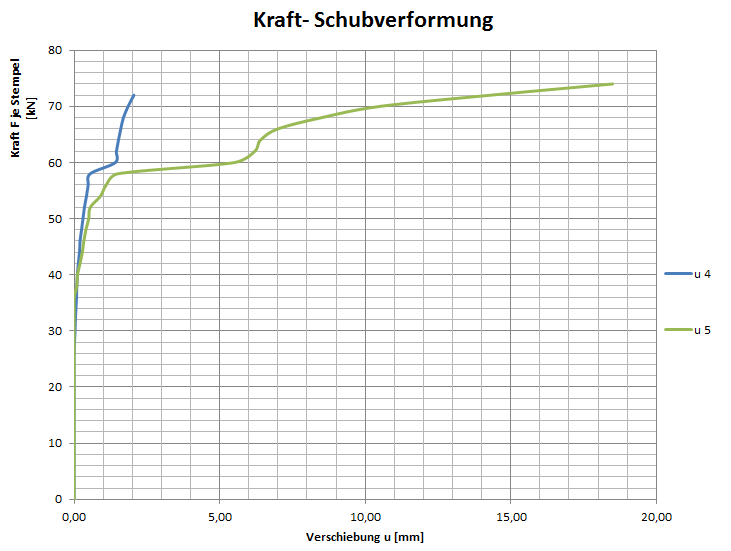
\includegraphics[scale =0.9]{1_versuch_kraft_schubverschiebung.png}
\caption{1 Versuch: Kraft-Schubverformung}
\label{1_versuch_kraft_schubverschiebung}
\end{center}
\end{figure}

In der Abbildung \ref{1_versuch_kraft_schubverschiebung} wird die relative Verschiebung zwischen der CLT-Schicht und der Betonschicht gezeigt. Es ist auch in diesem Diagramm erkennbar, das bei 58 kN der Verbund zwischen der CLT-Schichten und der Holzbetonschicht nicht mehr vorhanden war. Der Ausschlag der Kennlinie u 5 ist um ein vielfaches größer, da auf dieser Seite des Träger, die Keilzinkung versagte. 

\subsection{Schubversuch}


In einem ersten Schritt des Versuchskörpers wurde der gesamte Träger abgedrückt, mit dem 4-Punktbiegeversuch. Der Träger wurde nur auf einer Seite zerstört, auf der anderen Seite waren keine Beschädigungen ersichtlich. Somit wurde ein weiterer Verwendungszweck gesucht, um den nicht beschädigten Trägerteil zu nutzen. In der Abbildung \ref{träger_scherversuch}. ist ersichtlich welche Teile des Trägers verwendet wurden. 


\begin{figure}[h]
\begin{center}
\includegraphics[scale =0.9]{träger_scherversuch.png}
\caption{Darstellung des verwendeten Teiles der Trägers}
\label{träger_scherversuch}
\end{center}
\end{figure}

\paragraph{Erklärung des Schubversuchs}

\begin{figure}
\begin{minipage}[hbt]{8cm}
	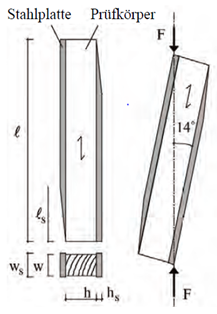
\includegraphics[width=5cm]{versuchsschema_scherversuch.png}
	\caption{Versuchsschema: Scherversuch }
	\label{versuchsschema_scherversuch}
\end{minipage}
\hfill
\begin{minipage}[hbt]{8cm}
Die Ermittlung von Scher- bzw. Schubfestigkeiten für den Holz und vor allem für  Sandwichbauteil existiert die Problematik, dass es nahezu unmöglich ist, einen reinen Schubspannungszustand zu erzeugen. Durch die geringe innere Festigkeit des Velox, sind die gängigen Prüfverfahren nicht anwendbar. 
Im Wesentlichen haben sich heute zwei Prüfverfahren zur Ermittlung der Schubfestigkeit von Holz etabliert, welche den einschlägigen Normen in verschiedenen Ländern zugrunde liegen. Im Europäischen Raum bezieht sich der [DIN EN 1995-1-1] auf die [DIN EN 408] wo das in Prüfverfahren erläutert wird. Dieser Versuchsaufbau wurde von uns adaptiert um das Verformungsverhalten der Verbundfuge zu untersuchen. Bei unserem Sandwichbauteil kommt anstatt der Stahlplatte, zum einem eine CLT-Platte und zum anderen eine SCC-Schicht zum Einsatz.

\end{minipage}
\end{figure}

\clearpage{}

Der Vorteil dieses Versuchsaufbaus liegt darin, dass der Bauteil in keiner Richtung gehalten werden muss und somit keine Querkräfte ableitet werden. Es wird die aufgebrachte Kraft, durch die Verbundfuge des Bauteils abgeleitet.

\paragraph{Abemessungen und Versuchsdarstellung}





\begin{enumerate}
\item Versuch: 150 x 50 x 32,8 cm
\item Versuch: 100 x 50 x 32,8 cm
\end{enumerate}

\begin{figure}
\begin{minipage}[hbt]{7cm}	
	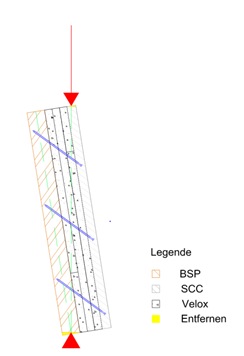
\includegraphics[width=8cm]{versuchsdarstellung_scherversuch_zeichnung.png}
	\caption{Zeichung der Scherversuchdarstellung}
	\label{Zeichung der Scherversuchdarstellung}
\end{minipage}
\hfill
\begin{minipage}[hbt]{7cm}
	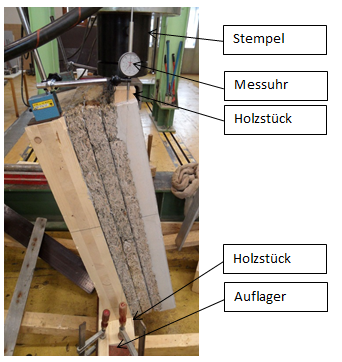
\includegraphics[width=8cm]{versuchsdarstellung_scherversuch_real.png}
	\caption{Darstellung des Scherversuchs}
	\label{Darstellung des Scherversuchs}
\end{minipage}
\end{figure}




\begin{figure}[h]
\begin{minipage}[hbt]{8cm}
	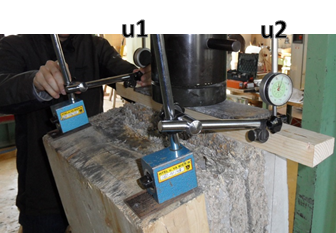
\includegraphics[width=5cm]{messeinrichtung_scherversuch.png}
	\caption{Anordnung und Darstellung der Messmittel }
	\label{messeinrichtung_scherversuch}
\end{minipage}
\hfill
\begin{minipage}[hbt]{8cm}
Es wurden für den Versuch 2 Messuhren am oberen Punkt des Bauteils mittels einer Stahlplatte angebracht. Somit konnte die Relativverschiebung zwischen der CLT- Schicht und der SCC-Schicht gemessen werden.

\end{minipage}
\end{figure}

\paragraph{Versuchsablauf und Messeinrichtung}
 
Damit der Versuchsbauteil die schräge Lage einnimmt, wurde Holzstücke entsprechend der Neigungen angefertigt. Aufgrund der Unterschiedlichen Höhen der Versuchskörper waren diese Holzstücke unterschiedlich. Um ein verrutschen des Holzauflagers zu verhindern, wurden Befestigungszangen verwendet.
Zu Beginn des Versuchs wurde eine Referenzkraft von 0,5 kN aufgebracht. Die Messuhren wurden anschließend auf Null zurückgestellt.
Die Kraft wurde mit einer Geschwindigkeit von 1kN pro 10 Sekunden aufgebracht. Um die Verschiebung messen zu können sind Messuhren verwendet worden. Das Ablesen der Verschiebung erfolgte manuell von den Messuhren.

\begin{figure}
\begin{minipage}[hbt]{7cm}	
	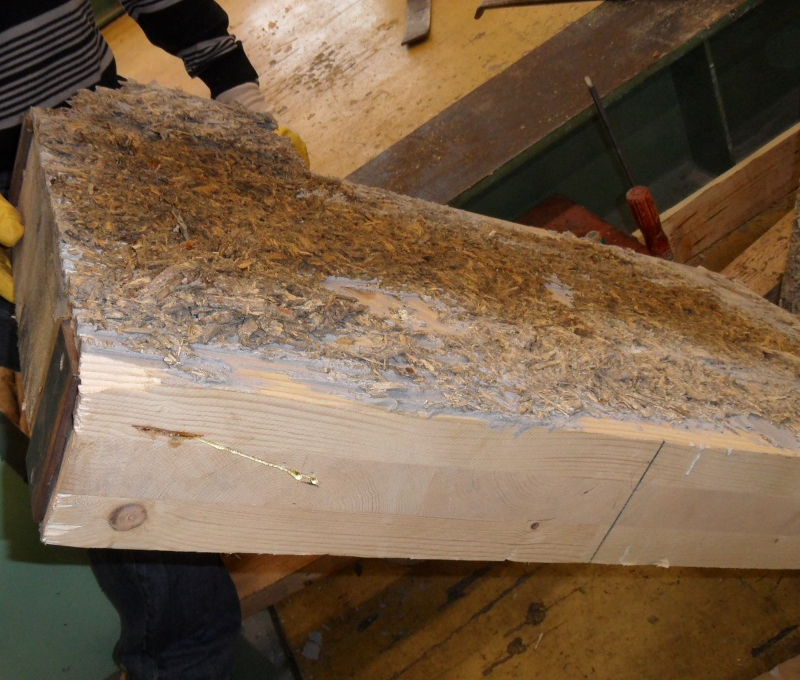
\includegraphics[width=8cm]{bruchbild1_scherversuch.png}
	\caption{bruchbild scherversuch}
	\label{bruchbild scherversuch}
\end{minipage}
\hfill
\begin{minipage}[hbt]{7cm}
	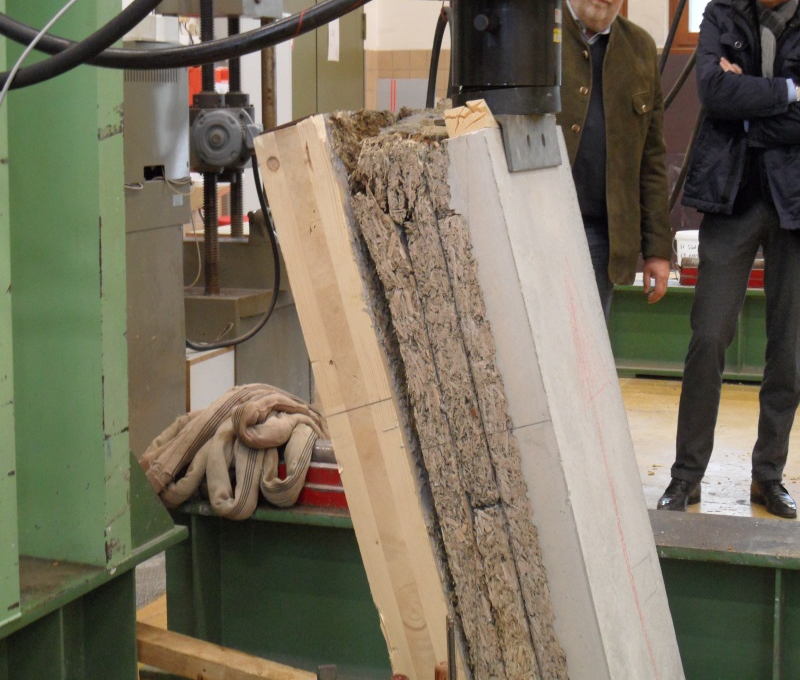
\includegraphics[width=8cm]{bruchbild2_scherversuch.png}
	\caption{bruchbilder scherversuch}
	\label{bruchbilder scherversuch}
\end{minipage}
\end{figure}

Auf den Bruchbildern ist erkennbar, dass die innere Festigkeit des Velox in der Verbundfuge zwischen der CLT-Schicht und dem Holzbeton versagt hat. Der Kleber ist nur gering in das Velox eingedrungen und hat somit wenige Bestandteile gebunden. Es sind teilweise Stellen erkennbar, die keinen oder nur geringen Anteil des Holzbetons aufweisen haben. Dies ist auf Verarbeitungsmängel zurückzuführen. Bei dem Versuch wurden alle Schrauben aus dem CLT ausgezogen und keine wurde abgerissen. 


\paragraph{Auswertung des Schubversuchs}




\begin{table}
\caption{Maximalbelastung der Schubversuche}
\begin{center}

\begin{tabular}{|c|c|}
\hline 
Versuch & Bruchkraft  \\ 
\hline 
1 & 359 [kN] \\ 
\hline 
2 & 345 [kN] \\ 
\hline 
\end{tabular} 


\end{center}
\end{table}




\begin{figure}
\begin{center}
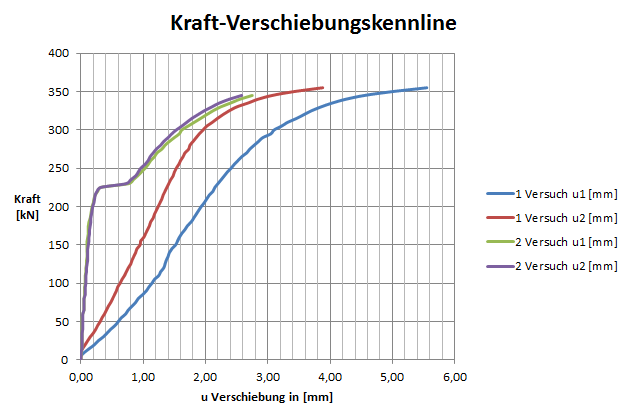
\includegraphics[scale =0.9]{Scherversuch_Kraft_Verschiebungslinie.png}
\caption{Scherversuch Kraft Verschiebungslinie}
\label{Scherversuch Kraft Verschiebungslinie}
\end{center}
\end{figure}

\subparagraph{Conclusio:}
Es ist ersichtlich das die beiden Versuche die fast gleiche Bruchlast aufweisen. Jedoch ist die Verschiebung beim 2 Versuch um die Hälfte geringer. Der Verlauf der Kennlinie ist auch nicht ident, daher müssten verschiedene Mechanismen bei den  Versuchen unterschiedlich aufgetreten sein. 
Der Hauptgrund für die unterschiedliche Kennlinie wird sein, die Vorbelastung durch den  4 Punktbiegeversuch. Auch wenn visuell keine Beeinträchtigung der Versuchskörper zu sehen war, hatte die Klebefuge bzw. die innere Festigkeit vom Velox, beim zweiten Versuch keinen Beitrag zur Lastabtragung. Somit musste die ganze Kraft über die Schrauben abgetragen werden.  Beim zweiten Versuch ist ein ausgeprägtes Plateau ersichtlich. Daher kann man davon ausgehen, dass vor dem Plateau die Schrauben und das Velox die Last abgetragen haben. Danach ist die Schraube alleine für die Lastabtragung verantwortlich. Die Steigung der Kennlinie bekräftigt die die oben beschriebene Vermutung, dass das System steifer ist als beim ersten Versuch. Beim zweiten Versuch ist die kein Plateau ersichtlich daher keine Beitrag vom Velox und somit eine geringe Steifigkeit des Systems.
Der Unterschied in den Verschiebung könnte durch die beschriebenen Steifigkeitsunterschiede abgeleitet werden. Die Schrauben werden beim 2 Versuch noch durch die intakte Verbundfuge 
unterstützt, daraus ergibt sich eine geringere Verschiebung in der ersten Phase des Versuchs.



\begin{figure}
\begin{center}
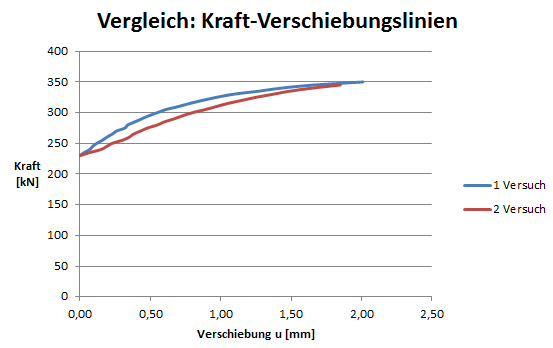
\includegraphics[scale =0.9]{Vergleich_Schubersuch.png}
\caption{Vergleich der Kennlinien nach 230 kN}
\label{VergleichSchubersuch}
\end{center}
\end{figure}

Vergleicht man die Kennlinien explizit nur in der Phase nach dem Plateau bzw. ab der Stelle, wo nur noch die Schrauben zur Lastableitung beitragen, ist die Kennlinie nahezu ident. Das heißt der Unterschied zwischen den Versuchskennlinien, kann auf die unterschiedliche Ausganglage (Vorschädigung) der Versuchskörper zurückführt werden. 


\section{2 Versuch}

\subsection{Anmerkung:}

Der Schichtenaufbau ist wie im Kapitel ..3 beschrieben. Die Anordnung der Schrauben ist aus der Abbildung \ref{2versuch} zu entnehmen. Es wurde wie in der Tabelle \ref{tab:Versuchsprogramm}  aufgelistet, der Kleber ElastoCem 109 verwendet für die Probe verwendet. Die Belastungsgeschwindigkeit betrug 4 [kN/min].
\begin{figure}
\begin{center}
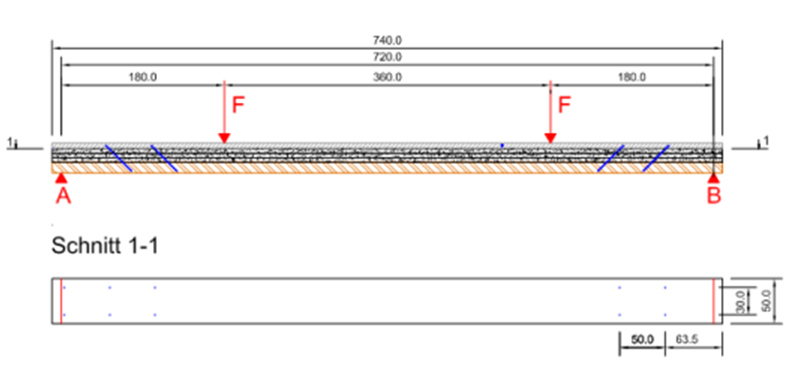
\includegraphics[scale =0.8]{2versuch.png}
\caption{Darstellung des Versuchskörpers}
\label{2versuch}
\end{center}
\end{figure}



\subsection{Vorbemerkung}

Der Versuchskörper hat wie in den Abbildungen \ref{schädigung scc} und \ref{schädigung velox} dargestellt, einige Schädigungen aufgewiesen. Es sind die Ergebnisse daher mit Vorsicht zu sehen. Auf den beiden Enden des Bauteil hatte sich die obersten Schichten der Veloxplatten von einander abgehoben. Weiters waren noch Risse in der Betonschicht im Bereich der 1/4 Punkte zu erkennen.
Die Schädigung sind beim Einlegen des Trägers in die Prüfanlage aufgetreten. Der Träger wurde mit 2 Gurten, eher mittig, angehoben und erfuhr daher einen Lastzustand der nicht vorgesehen war. Durch das mittige Anhebung war ein Kragarm and den Enden  mit ca. 2,50 $m$ Länge entstanden. Womit sich die Zug und Druckzone umgekehrte. So entstanden die Risse im Beton. Das Abheben der oberen Veloxschichten ist auf den verwendeten Kleber zurückzuführen. Er hatte zu geringe Klebeeigenschaften und es wurde laut einer Expertenaussage (Hr. Rössler)  der Kleber zu gering aufgetragen.
Es ist noch festzuhalten das beim 1 Bauteilversuch ident vorgegangen worden ist. Aufgrund der Verringerung der Schraubenanzahl und der Verwendung eines anderen Klebers, ist ein Bauteil entstanden, der eine geringe Steifigkeit hat. Dies ist der Grund für die Schädigung des Bautteils.




\begin{figure}[h]
\begin{minipage}[hbt]{7cm}	
	\includegraphics[width=8cm]{schädigung_velox.jpg}
	\caption{schädigung velox}
	\label{schädigung velox}
\end{minipage}
\hfill
\begin{minipage}[hbt]{7cm}
	\includegraphics[width=8cm]{schädigung_scc.jpg}
	\caption{Schädigung des Betons}
	\label{schädigung scc}
\end{minipage}
\end{figure}


\subsection{Versagensbeschreibung und Auswertung}



\begin{figure}
\begin{center}
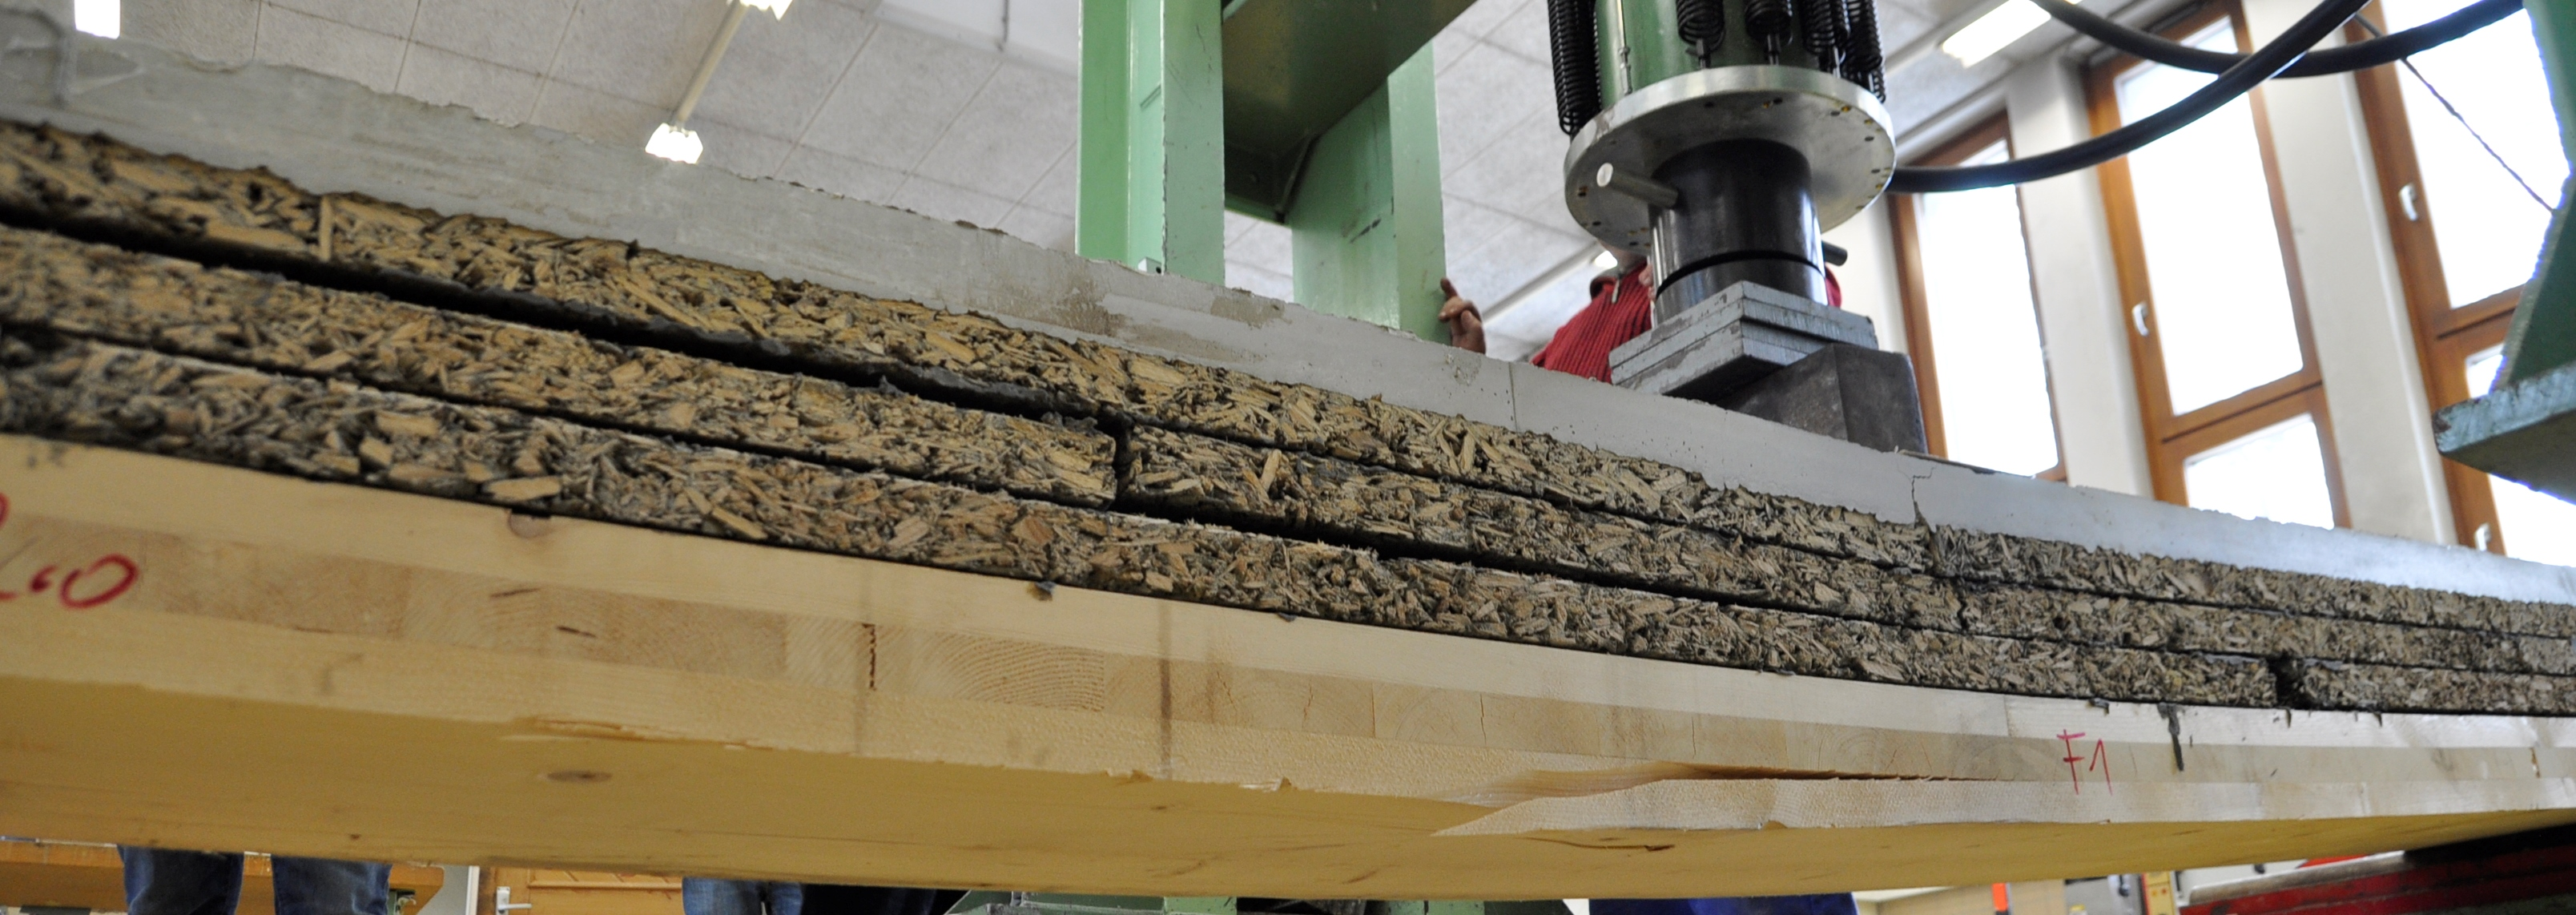
\includegraphics[scale =0.5]{2versuch_versagen.jpg}
\caption{Darstellung des Versagen}
\label{2versuch versagen}
\end{center}
\end{figure}

In der Abbildung \ref{2versuch versagen} sind die maßgebenden Schädigungen abgebildet, die beim Versuch aufgetreten sind. Es ist ein Riss im Beton, im Bereich der Lasteinleitung zu sehen, der jedoch schon vor dem Versuch entstand. Es ist ist weiters zu erkennen, dass die Veloxschichten in der Mitte des Träger keinen Verbund hatten und sich von einnander abhoben. Der Riss in der CLT-Platte ist bei der Laststufe von ca 22kN aufgetreten. \\

\begin{figure}[h]
\begin{minipage}[hbt]{7cm}	
	\includegraphics[width=7cm]{2versuch_1oberfläche_velox.jpg}
	\caption{Oberfläche der aufgetragenen Schicht}
	\label{velos unten}
\end{minipage}
\hfill
\begin{minipage}[hbt]{7cm}
	\includegraphics[width=7cm]{2versuch_2oberfläche_velox.jpg}
	\caption{Oberfläche der aufgelegten Schicht}
	\label{velox ober}
\end{minipage}
\end{figure}

In den Abblindungen \ref{velos unten} und \ref{velox ober} sind die Oberflächen abgebildet, die zur großen Fuge führten. Es sind Teilflächen zu erkennen, welche noch die Riffen der Zahnspachtel aufweisen und Teilflächen auf der gegenüber liegenden Seite, die keine Benetzung mit dem Kleber vorweisen. In diesen Bereich hat nie ein Verbund stattgefunden. Es liegt hier kein Versagen der Veloxschicht vor, ausschließlich von der Klebeschicht, da keine Spuren von der Veloxplatte auf der unteren feststellbar  


\begin{figure}
\begin{center}
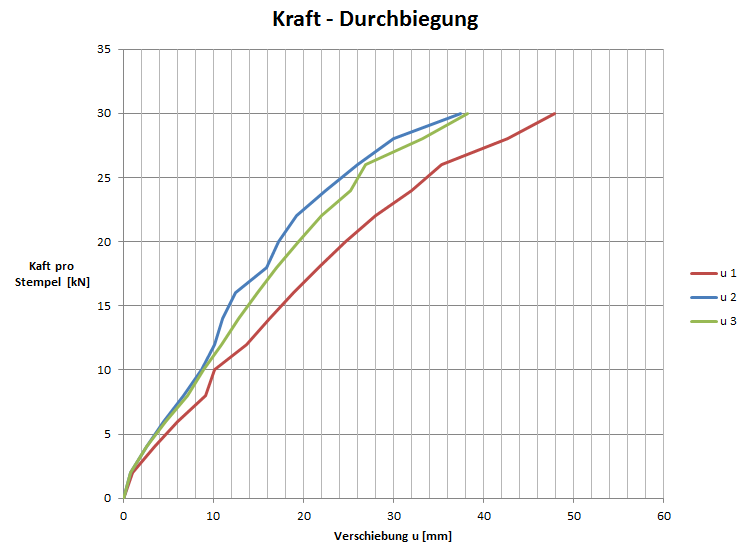
\includegraphics[scale =0.6]{2versuch_kraft_durchbiegung.png}
\caption{2 Versuch: Kraft-Durchbiegung}
\label{2 Versuch: Kraft-Durchbiegung}
\end{center}
\end{figure}



\begin{figure}
\begin{center}
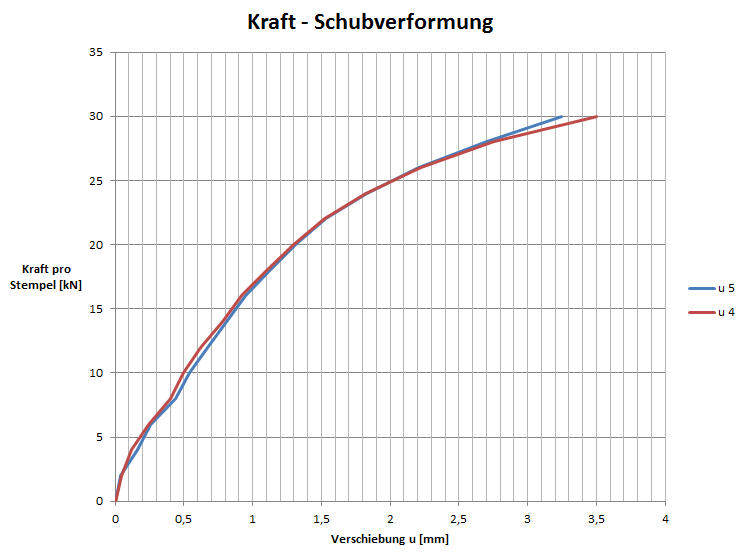
\includegraphics[scale =0.6]{2versuch_kraft_schubverformung.png}
\caption{2 Versuch: Kraft-Schubverformung}
\label{2_versuch_kraft_schubverschiebung}
\end{center}
\end{figure}

Die Verschiebungslinie u 1 ist in der Mitte des Trägers gemessen und legt bis zu 25 kN ein lineares Verhalten vor. Die Sprung bei 8 kN bzw bei 10 kN wird durch das Ablesen bedingt sein. Nach den 25 kN ist die Kennlinie deutlich flacher daher wird der gesamte Verbund von der Zwischenschicht (Velox) nicht mehr gegeben sein. Die weitere Laststufe wird durch die Schrauben aufgenommen. Eine weitere Laststeigerung war nicht mehr möglich, daher ist es schwierig zu sagen, ab welchen Zeitpunkt die Schrauben komplett ausgerissen sind.
Die Kennlinien der Messpunkte u 2 und u 3 sind bin zu 10 kN ident, danach sind schon Unterschiede in der Verformung erkennbar. Die Unterschiede können wiederum auf die manuelle Auswertung geführt werden. Im Versuchsablauf waren  keine unsymmetrischen Schädigungen aufgetreten oder erkennbar. Bei der Last von 26 kN ist in der Kennlinie u 3 ein markanter Knick aufgetreten, der in der an auch bei der Kennlinie u 1 aufgetreten ist. 

Die relative Verschiebung zwischen der CLT-Schicht und der Betonschicht ist in de der Abbildung \ref{2_versuch_kraft_schubverschiebung}. Die Arbeitslinien sind nahezu ident. Sie weisen bis zu 20 kN ein nahezu lineares verhalten auf, danach ist ein progressiver Anstieg erkennbar.

\section{3 Versuch}

\subsection{Anmerkung:}
Der Schichtenaufbau ist wie im Kapitel 3 beschrieben. Die Anordnung der Schrauben ist aus der Abbildung \ref{3versuch} zu entnehmen. Es wurde wie in der Tabelle..  aufgelistet, der Kleber Sikatop 107 verwendet. Die Belastungsstufen sind im Kapitel 3.7 angegeben bzw können sie der Versuchsauswertung entnommen werden

\begin{figure}
\begin{center}
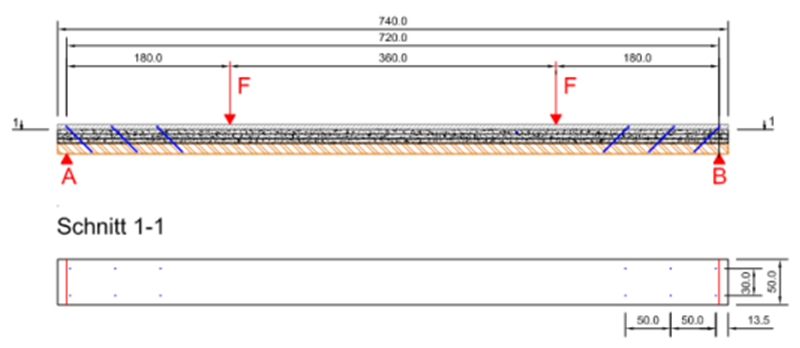
\includegraphics[scale =0.8]{3versuch.png}
\caption{Darstellung des Versuchskörpers}
\label{3versuch}
\end{center}
\end{figure}

\subsection{Versagensbeschreibung und Auswertung}

Der Bauteil hatte keine Beschädigungen vor dem Versuch.
Die ersten Schadenserscheinungen traten als Risse im Beton, im Bereich der Lasteinleitung, ein. In der Abbildung \ref{beton_veloxriss} ist der Riss ersichtlich. Weitere Schäden an dem Versuchskörper waren an der selben Stelle,in der Veloxschicht, erkennbar. Die Risse traten kurz vor dem erreichen der Höchstlast von 58 $ kN $ auf. In der Abbildund \ref{spalt} darstellt, ist ein Spalt, der im Laufe des Versuchs entstanden ist. Im Bereich zwischen der Lasteinleitung und dem Auflager B war ein Spalt von 1$ cm $ entstanden. 

\begin{figure}[h]
\begin{minipage}[hbt]{6cm}	
	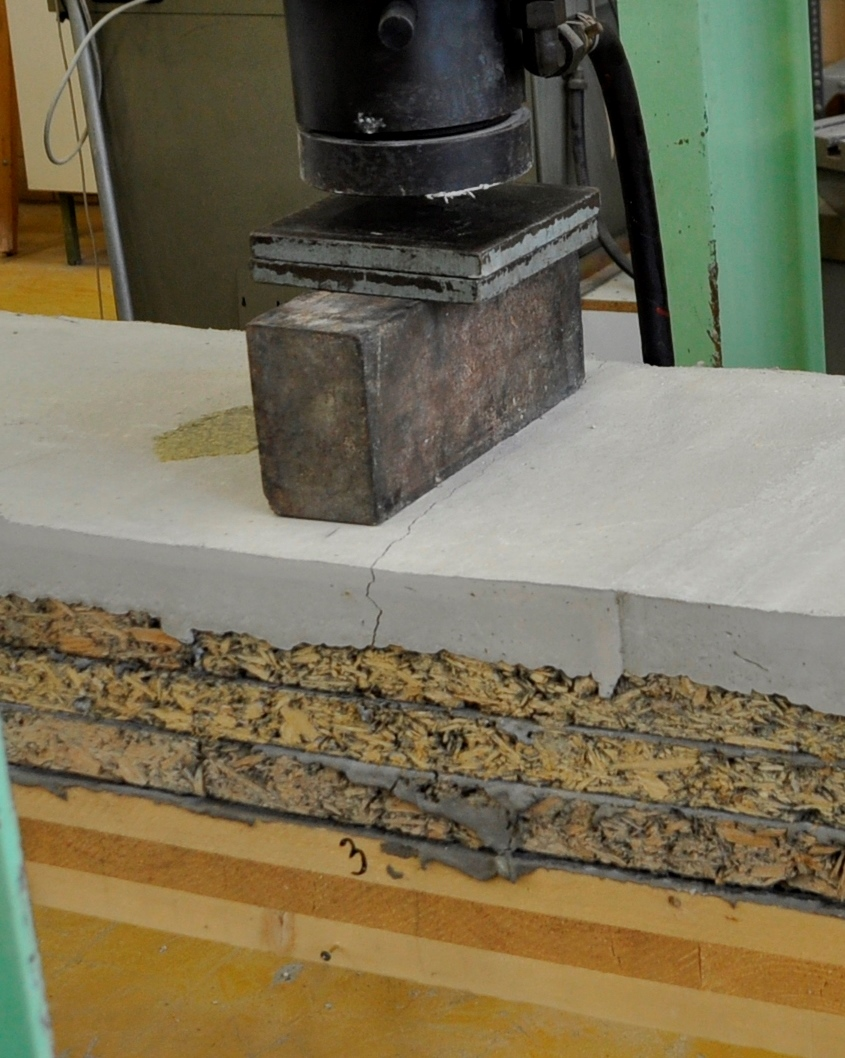
\includegraphics[width=6cm]{beton_veloxriss.jpg}
	\caption{Darstellung des Risse im Beton und Holzbeton}
	\label{beton_veloxriss}
\end{minipage}
\hfill
\begin{minipage}[hbt]{8cm}
	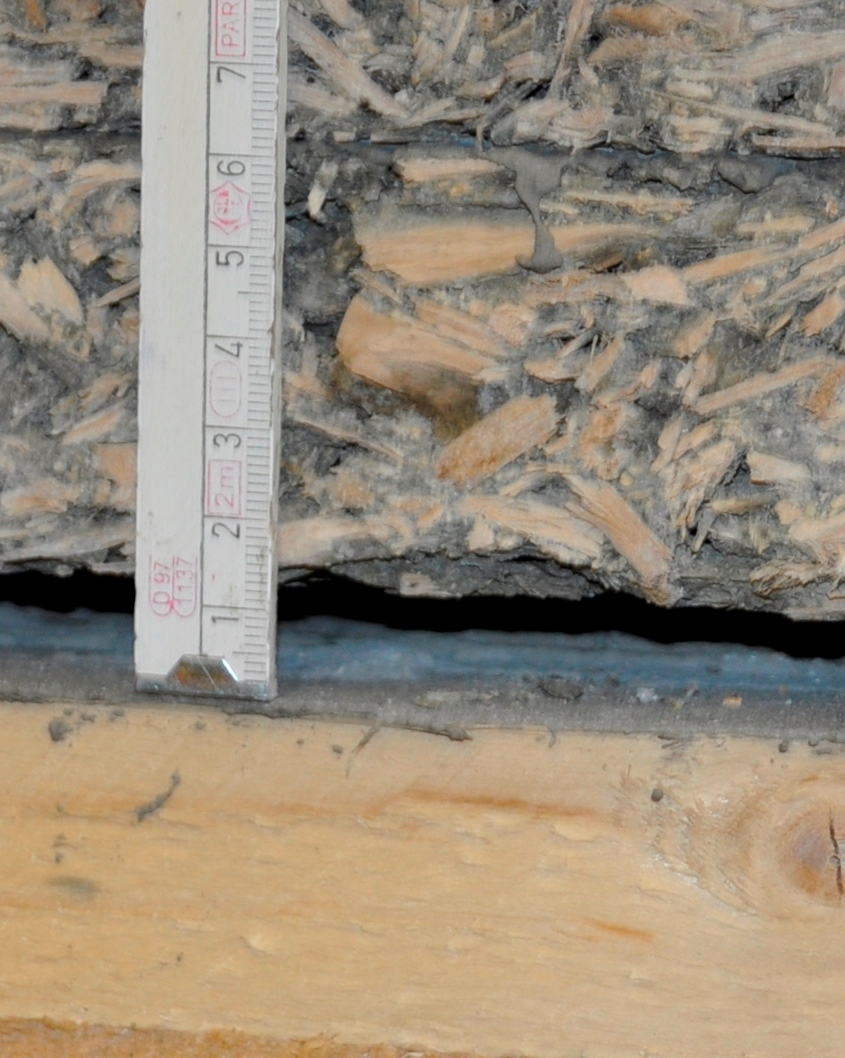
\includegraphics[width=8cm]{fuge.jpg}
	\caption{Spalt zwischen CLT und Holzbeton}
	\label{spalt}
\end{minipage}
\end{figure}


\begin{figure}
\begin{center}
	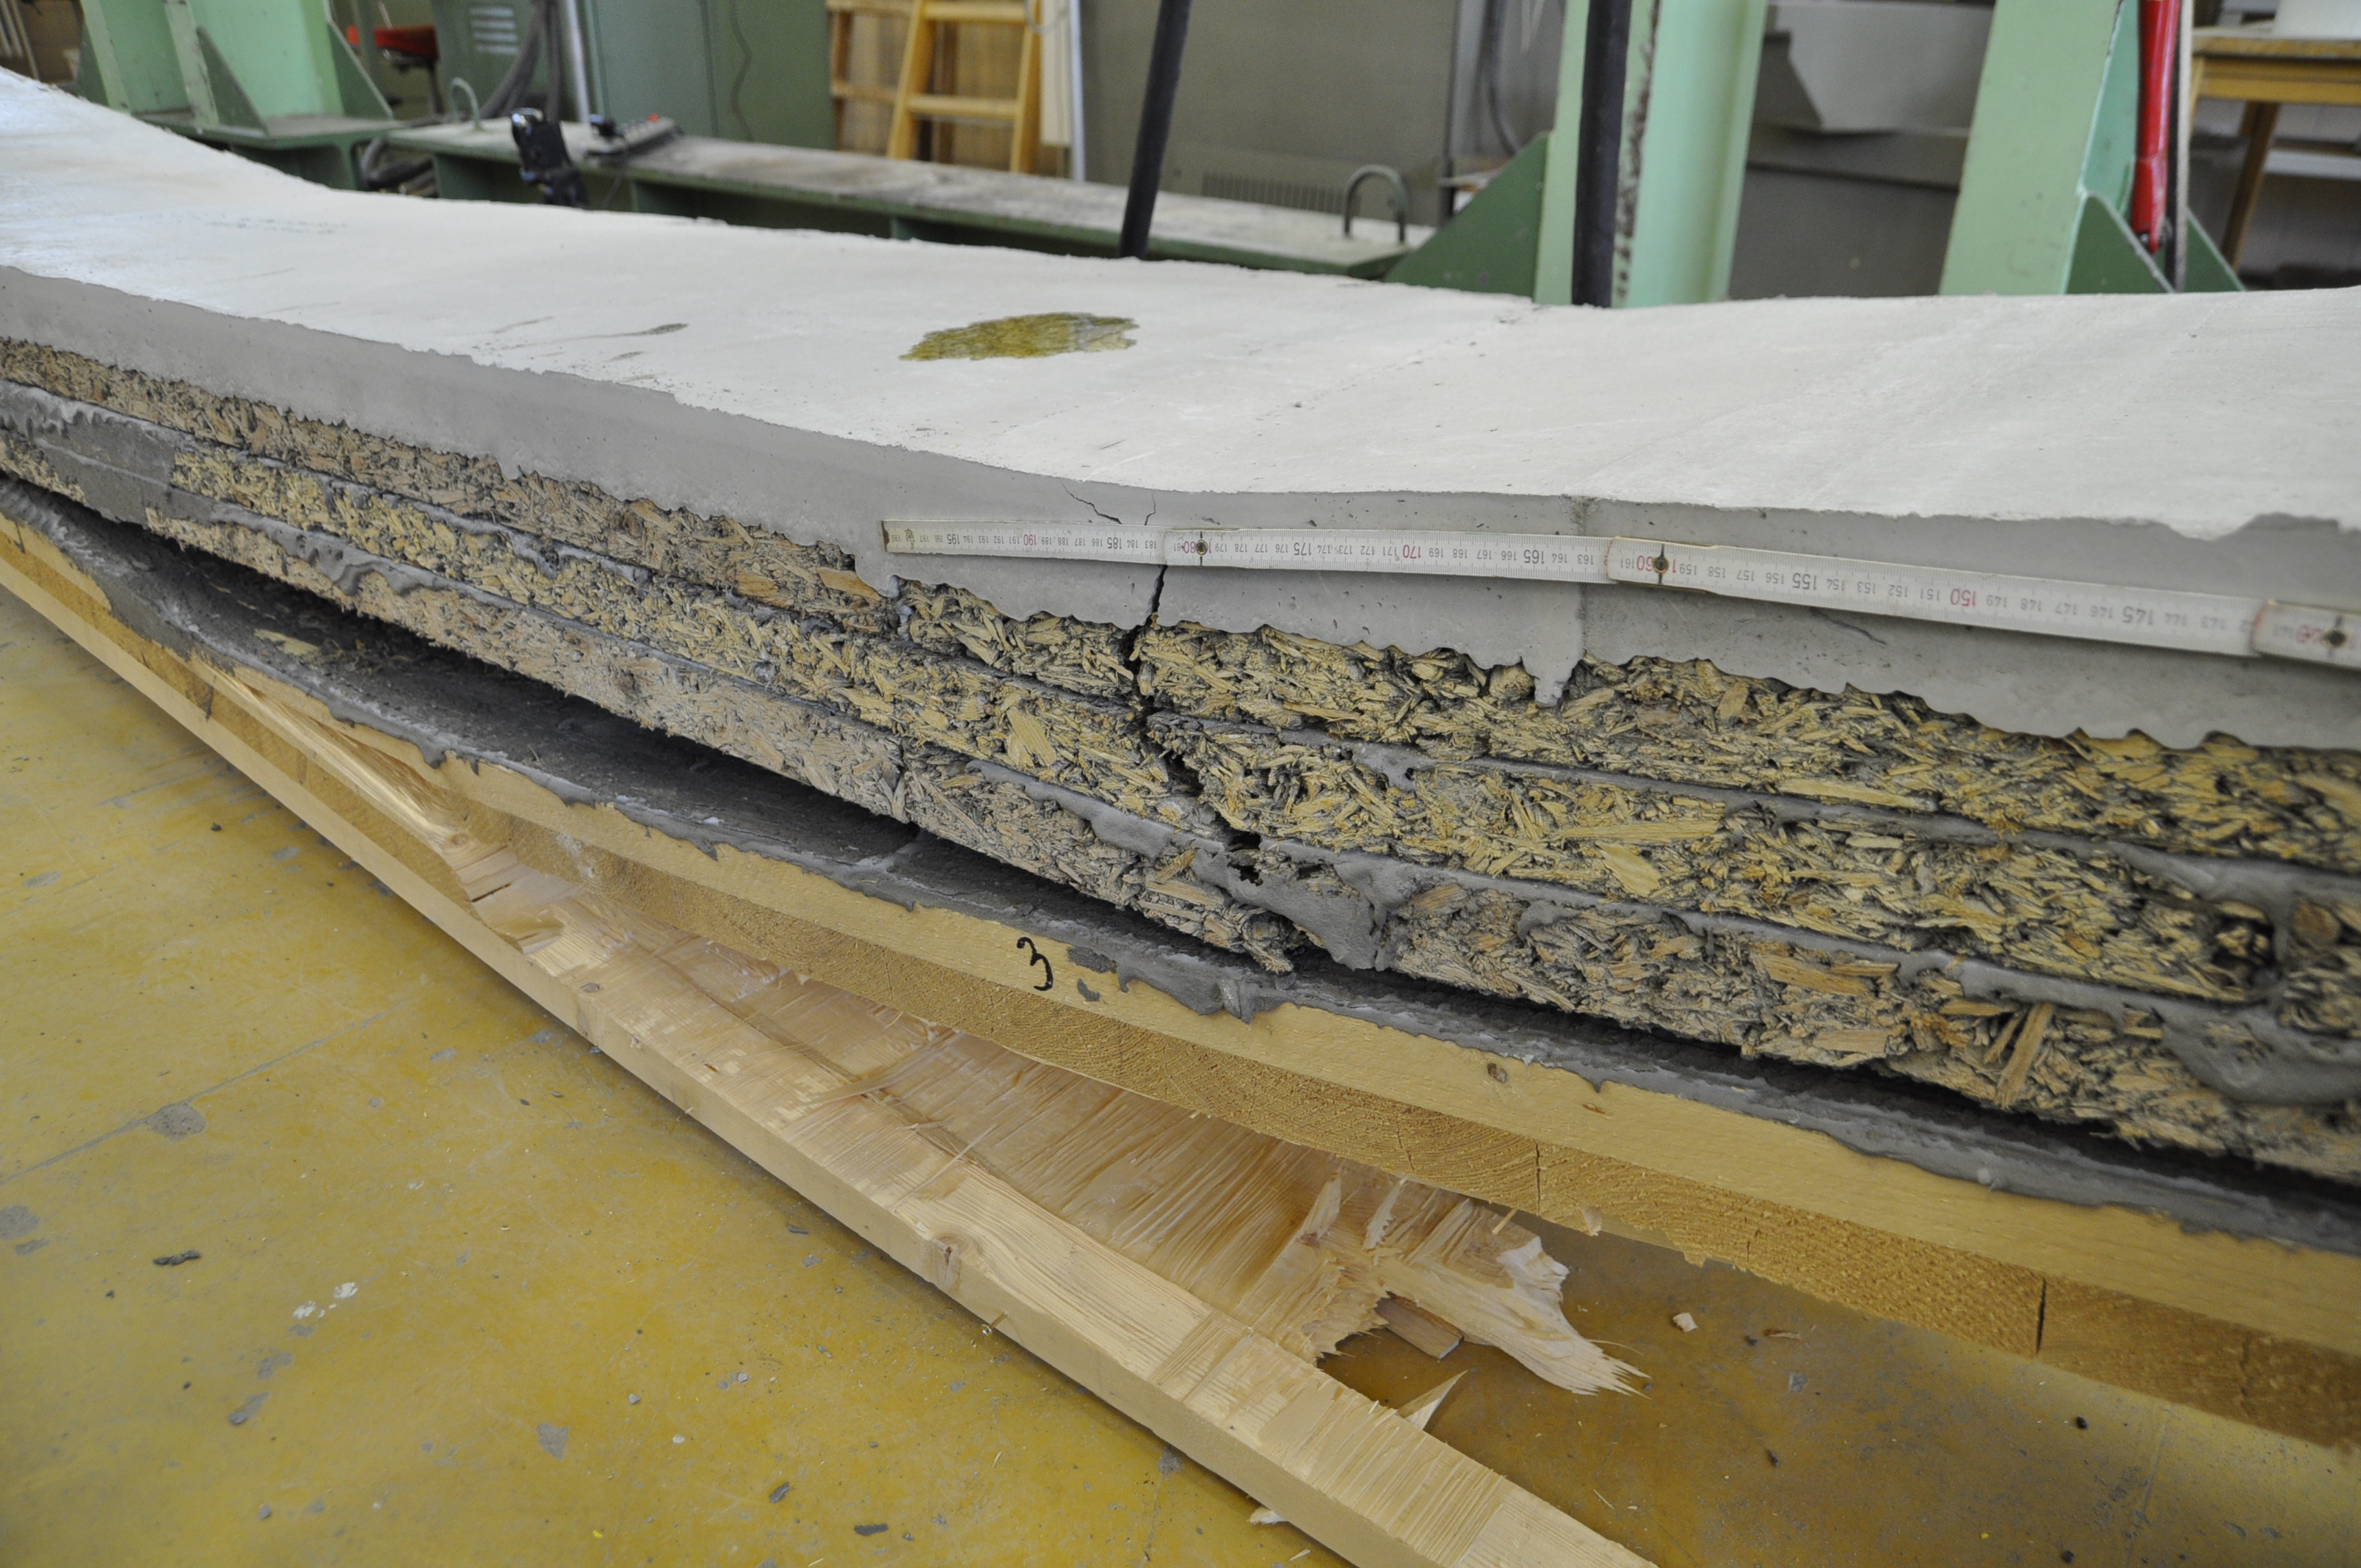
\includegraphics[scale=0.1]{bruch_3versuch.jpg}
	\caption{Bruch nach Wiederbelastung }
	\label{bruch_3versuch}
\end{center}
\end{figure}

Nach dem ersten Versagen und der Erreichung der maximalen Last, wurde der Bauteil  nochmals belastet. Durch den nicht intakten Verbund ergab sich eine Bruchlast von 40  $ kN $. In der Abbildung \ref{bruch_3versuch} ist die Bruchstelle nahe der Krafteinleitung dargestellt. Man erkennt die Risse von der oberen Betonschicht bis zur letzten Holzbetonschicht.In diesem Bereich wurde nach dem Bruch ein Asteinschluss festgestellte, womit eine weitere Schwachstelle entdeckt wurde.\\


\begin{figure}
\begin{minipage}[hbt]{5cm}
	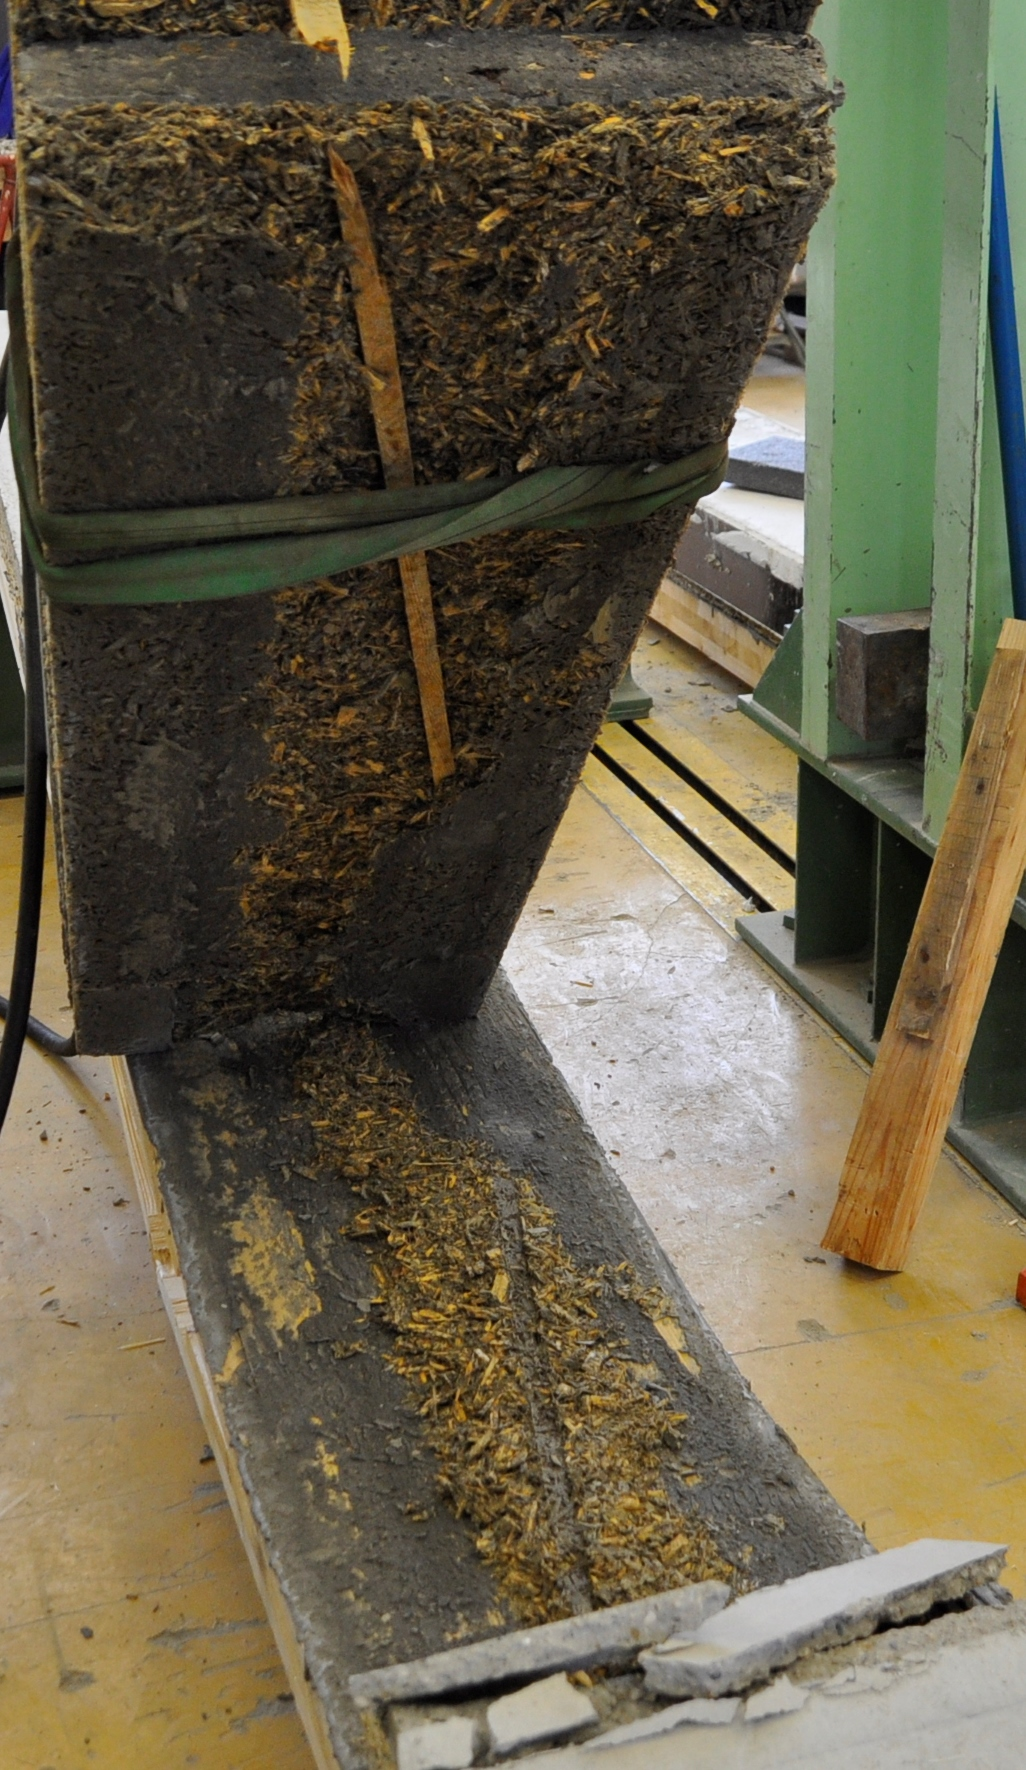
\includegraphics[width=6cm]{fugenbruch_3versuch.jpg}
	\caption{Oberflächbild: CLT-Platte und Holzspanbeton}
	\label{fugenbruch_3versuch}
\end{minipage}
\hfill
\begin{minipage}[hbt]{7cm}
Durch den Bruch konnte danach die Fuge zwischen Holzspanbeton und CLT-Platte betrachtet werden (Abbildung \ref{fugenbruch_3versuch}). Es zeigte sich, dass die in der Mitte des Bauteils der Holzbeton versagte hatte und in den Randzonen der Kleber zu geringe Vernetzung aufwies. Diese Auffälligkeit konnte auch an den Trägerenden beobachtet werden. Die Schrauben wurden in dem Versuch alle ausgezogen und keine zerstört.
Im weiteren sind geringe Flächen zu erkennen, wo die Haftung des Klebers auf der CLT-Platte zu gering war.  
\end{minipage}
\end{figure}




\begin{figure}
	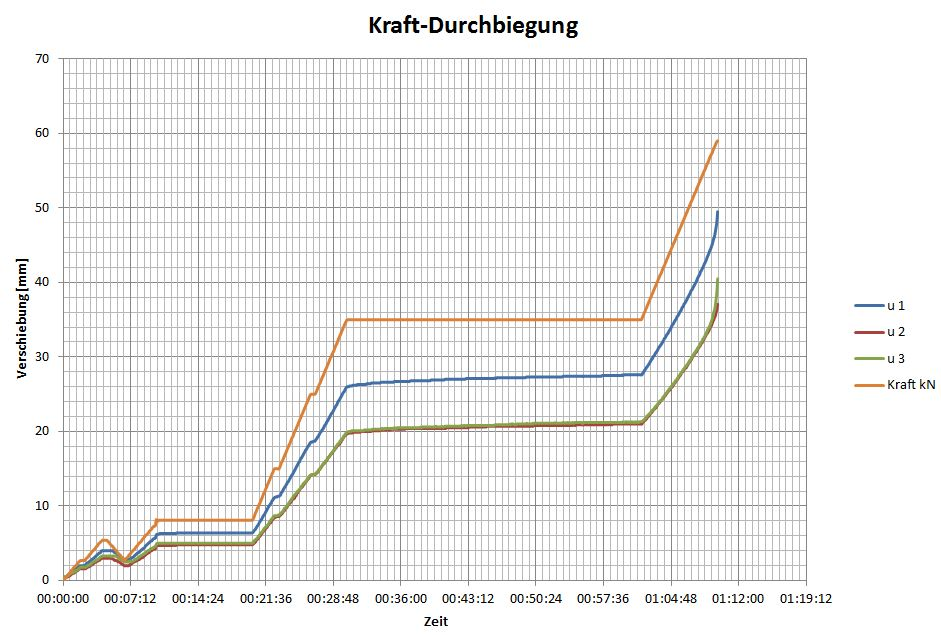
\includegraphics[scale=0.8]{3versuch_kraft_durchbiegung_zeit.jpg}
	\caption{3 Versuch: Kraft-Durchbiegung-Zeit}
	\label{3 Versuch: Kraft-Durchbiegung-Zeit}
\end{figure}




\begin{figure}	
	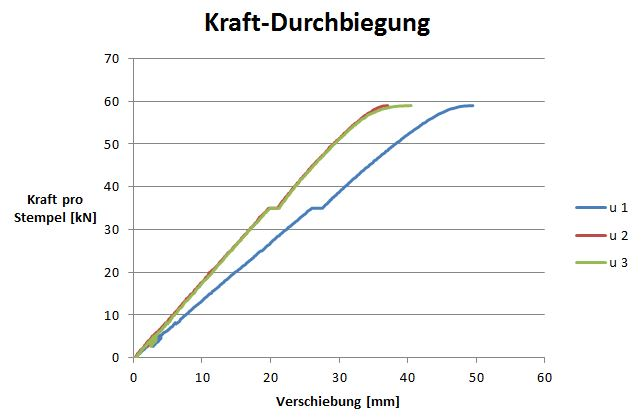
\includegraphics[scale=0.8]{3versuch_kraft_durchbiegung.jpg}
	\caption{3 Versuch: Kraft-Durchbiegung}
	\label{3 Versuch: Kraft-Durchbiegung}
\end{figure}





\begin{figure}	
	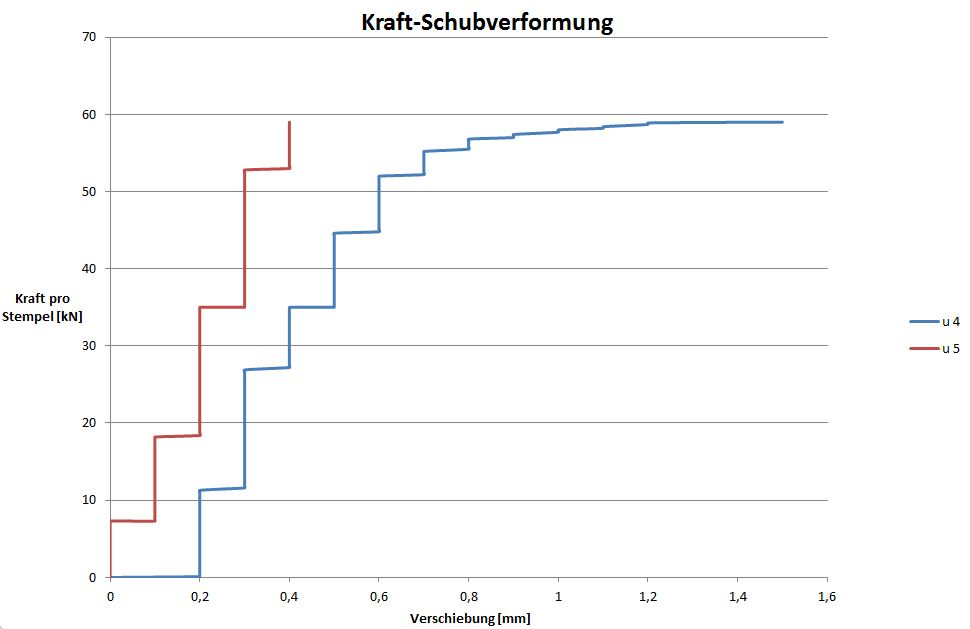
\includegraphics[scale=0.6]{3versuch_kraft_schubverformung.JPG}
	\caption{3 Versuch: Kraft-Schubverformung}
	\label{3 Versuch: Kraft-Schubverformung}
\end{figure}



In der Abbildung \ref{3 Versuch: Kraft-Durchbiegung} und \ref{3 Versuch: Kraft-Durchbiegung-Zeit} sind die Arbeitslinie der Kraft Durchbiegung bzw. bezogen auf die Zeit dargestellt. In der Abbildung \ref{3 Versuch: Kraft-Durchbiegung-Zeit} ist der Kraftverlauf darstellt, der wie in Kapitel 4.7 beschrieben ist. Die Kennlinien folgen dem Kraftverlauf, was auf einen linearen Verlauf hinweist. Dies ist auch in der Abbildung \ref{3 Versuch: Kraft-Durchbiegung} ersichtlich. Die Verschiebungen gehen bei dem Rückgang von 5,4 kN auf 2,7 kN auch zurück, deutet auf ein elastisches verhalten hin. Beim halten der Last von 8,1 kN ist keine Verschiebung erkennbar, somit auch kein Kriechen des Bauteils bei der Last. Nach der weiteren Belastung auf 35 kN sind zwei kleine Sprünge in der Lastkennlinie erkennbar, die sich auch in den Verschiebungslinien widerspiegeln. Bei dem Laststufe sind die ersten Risse im Beton und in weiterer Folge auch Risse im Velox entstanden. Bei der konstanten Last von 35 kN ist eine geringfügiger Anstieg  der Verschiebungskennlinien ersichtlich. Dies ist auf ein Kriechverhalten des Bauteils zurückzuführen.




In der Abbildung \ref{3 Versuch: Kraft-Schubverformung} ist die Schubverformung des Versuchs abgebildet. Durch die geringe Auflösung der Messaufnehmer, entstand die Treppenkurve. Bei Betrachtung der Kennlinie u5 ist erischtlich das hier bei den konstanten halten der Lasten (8,1 kN und 35 kN ) die Kurve einen entsprechenden Sprung in der Verschiebung aufweist, was auf eine Kriechverformung hinweist. Legt man eine Trend in die Arbeitslinien, ist ein annäherd linearer Verlauf bis zur Last von ca. 52 kN zu erkennen. 

\clearpage
\newpage
\section{4 Versuch}

\subsection{Anmerkung:}
Der Schichtenaufbau ist wie im Kapitel 3 beschrieben. Diese Probe wurde ohne Schrauben gefertigt,wie aus der Abbildung \ref{4versuch} zu entnehmen ist. Es wurde wie in der Tabelle \ref{tab:Versuchsprogramm}  aufgelistet, der Kleber Sikatop 107 verwendet. Die Belastungsstufen sind im Kapitel 3.7 angegeben bzw. können sie der Versuchsauswertung entnommen werden.

\begin{figure}[h]
\begin{center}
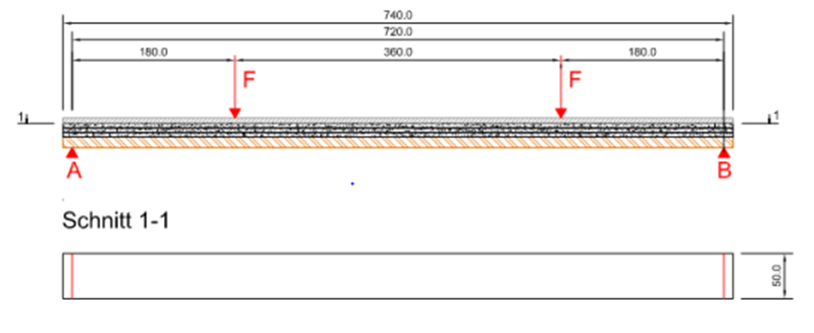
\includegraphics[scale =0.8]{4versuch.png}
\caption{Darstellung des Versuchskörpers}
\label{4versuch}
\end{center}
\end{figure}

\subsection{Vorbemerkung}

Der Versuchskörper hat wie in den Abbildungen \ref{riss} dargestellt, einige Schädigungen aufgewiesen. Es sind die Ergebnisse daher mit Vorsicht zu sehen. Auf den beiden Enden des Bauteil hatte sich die unteren Schichten der Veloxplatten von der CLT-Platte gelöst. Weiters wurden Risse in der Betonschicht im Bereich der 1/4 Punkte festgestellt.
Die Schädigung sind beim Einlegen des Trägers in die Prüfanlage aufgetreten. Der Träger wurde mit 2 Gurten angehoben und erfuhr daher einen Lastzustand der nicht vorgesehen war. Durch das Anhebung war ein Kragarm and den Enden  mit ca. 2,00 $m$ Länge entstanden. Womit sich die Zug und Druckzone umgekehrte. So entstanden die Risse im Beton. Das Abheben der oberen Veloxschichten ist auf den verwendeten Kleber zurückzuführen. Der Kleber hatte eine zu geringe Festigkeit, um die Eigenlast aufzunehmen. Ein weiterer Grund war, der Verzicht auf mechanische Verbindungsmittel, womit bei den anderen Versuchen keine Probleme vorhanden waren.

\begin{figure}
\begin{center}
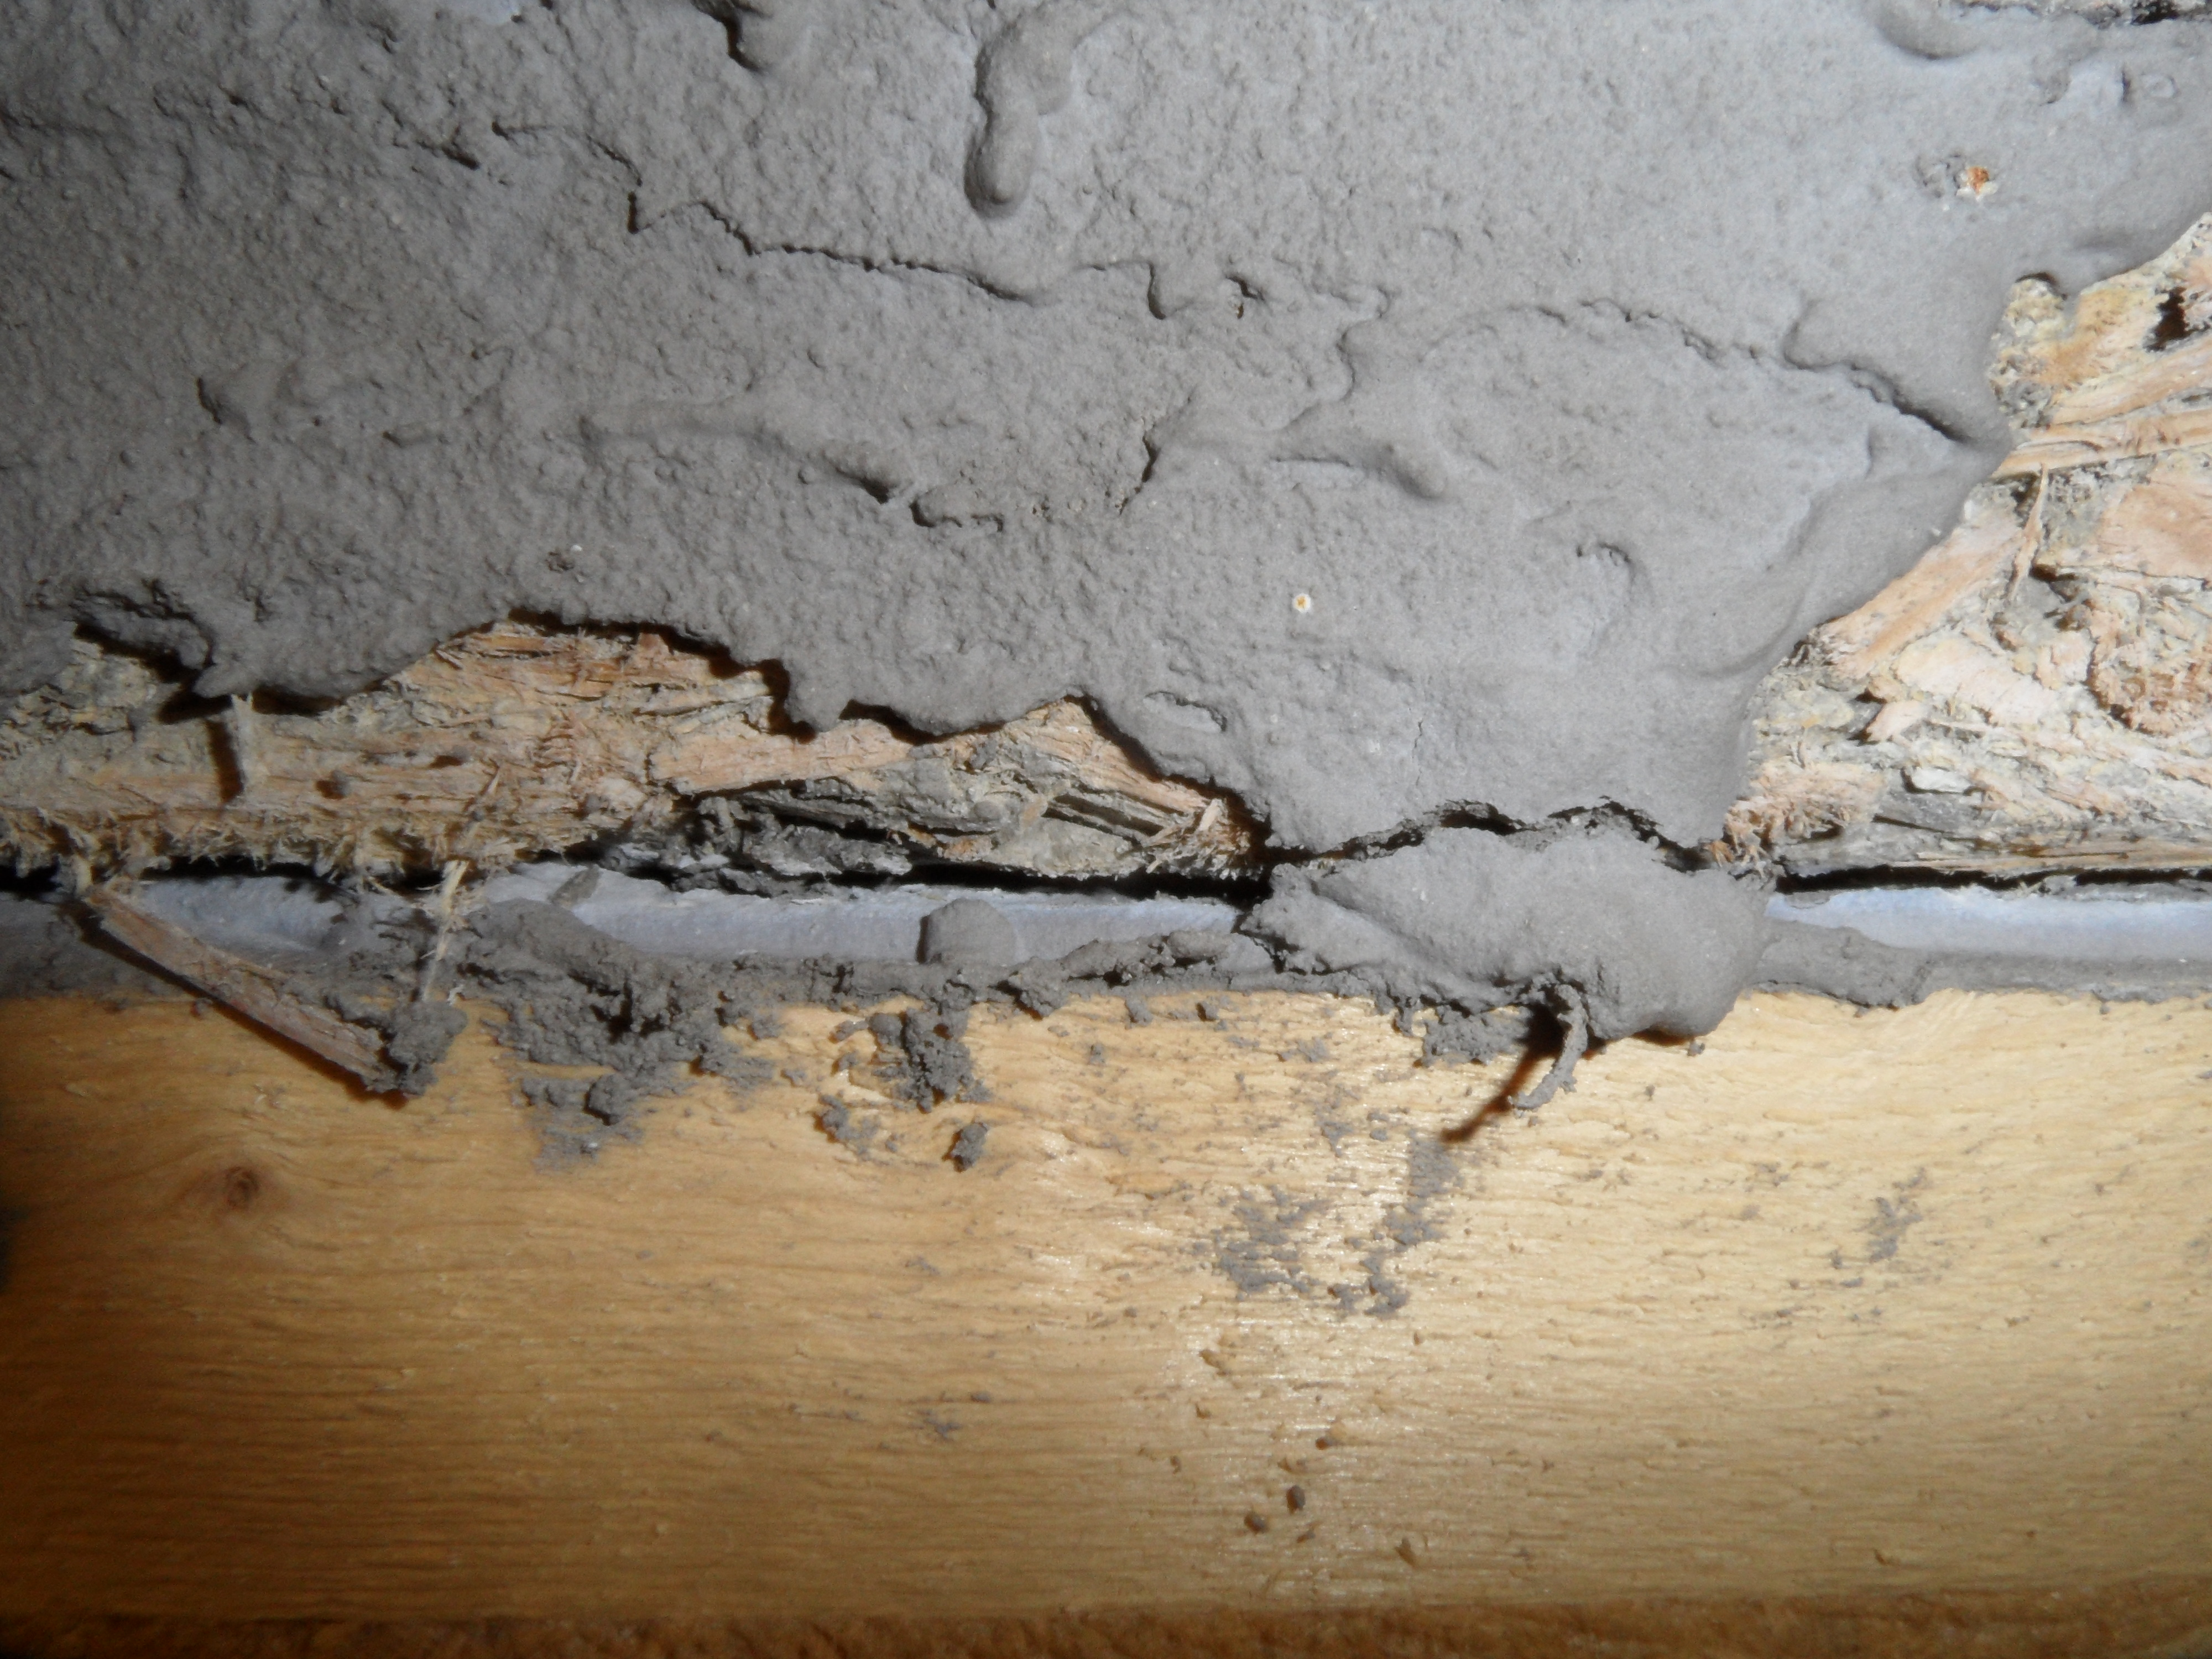
\includegraphics[scale =0.05]{riss.jpg}
\caption{Rissdarstellung in der unteren Klebefuge}
\label{riss}
\end{center}
\end{figure}


\subsection{Versagensbeschreibung und Auswertung}


In der Abbildung \ref{4versuch versagen} sind die maßgebenden Schädigungen abgebildet, die beim Versuch aufgetreten sind. Es ist eine horizontale Verschiebung beim Auflager A zu erkennen. Die Verschiebung der Fuge wurde hauptsächlich auf dieser  Auflagerseite A festgestellt. In der Abbildung \ref{4versuch_schichtbruch} sind Risse im Beton und in der Veloxschicht zu sehen, die im Bereich der Lasteinleitung entstanden sind. Schädigungen in der CLT-Platte waren keine erichtlich, die traten nach dem Versagen der oberen Schichten auf.  \\



\begin{figure}[h]
\begin{minipage}[hbt]{7cm}	
	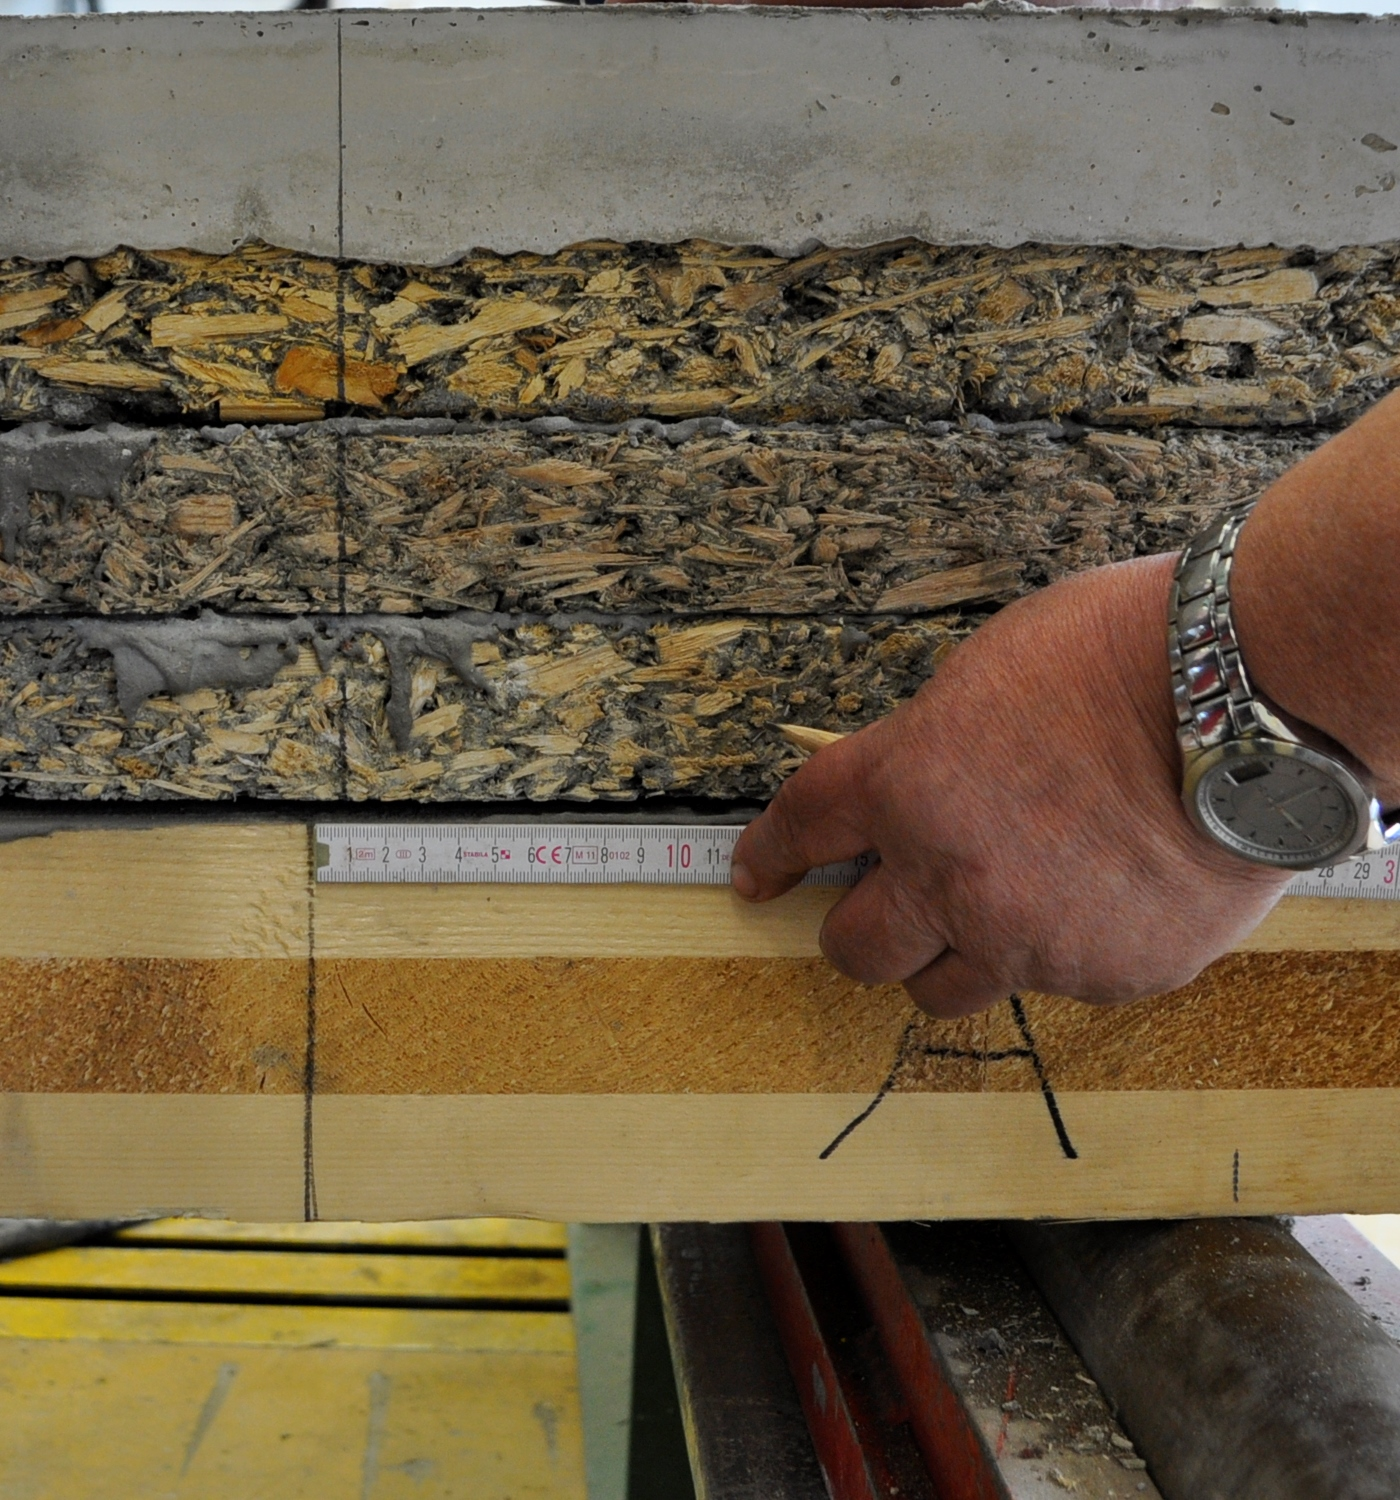
\includegraphics[width=7cm]{4versuch_versagen.jpg}
	\caption{Darstellung des Versagen}
	\label{4versuch versagen}
\end{minipage}
\hfill
\begin{minipage}[hbt]{7cm}
	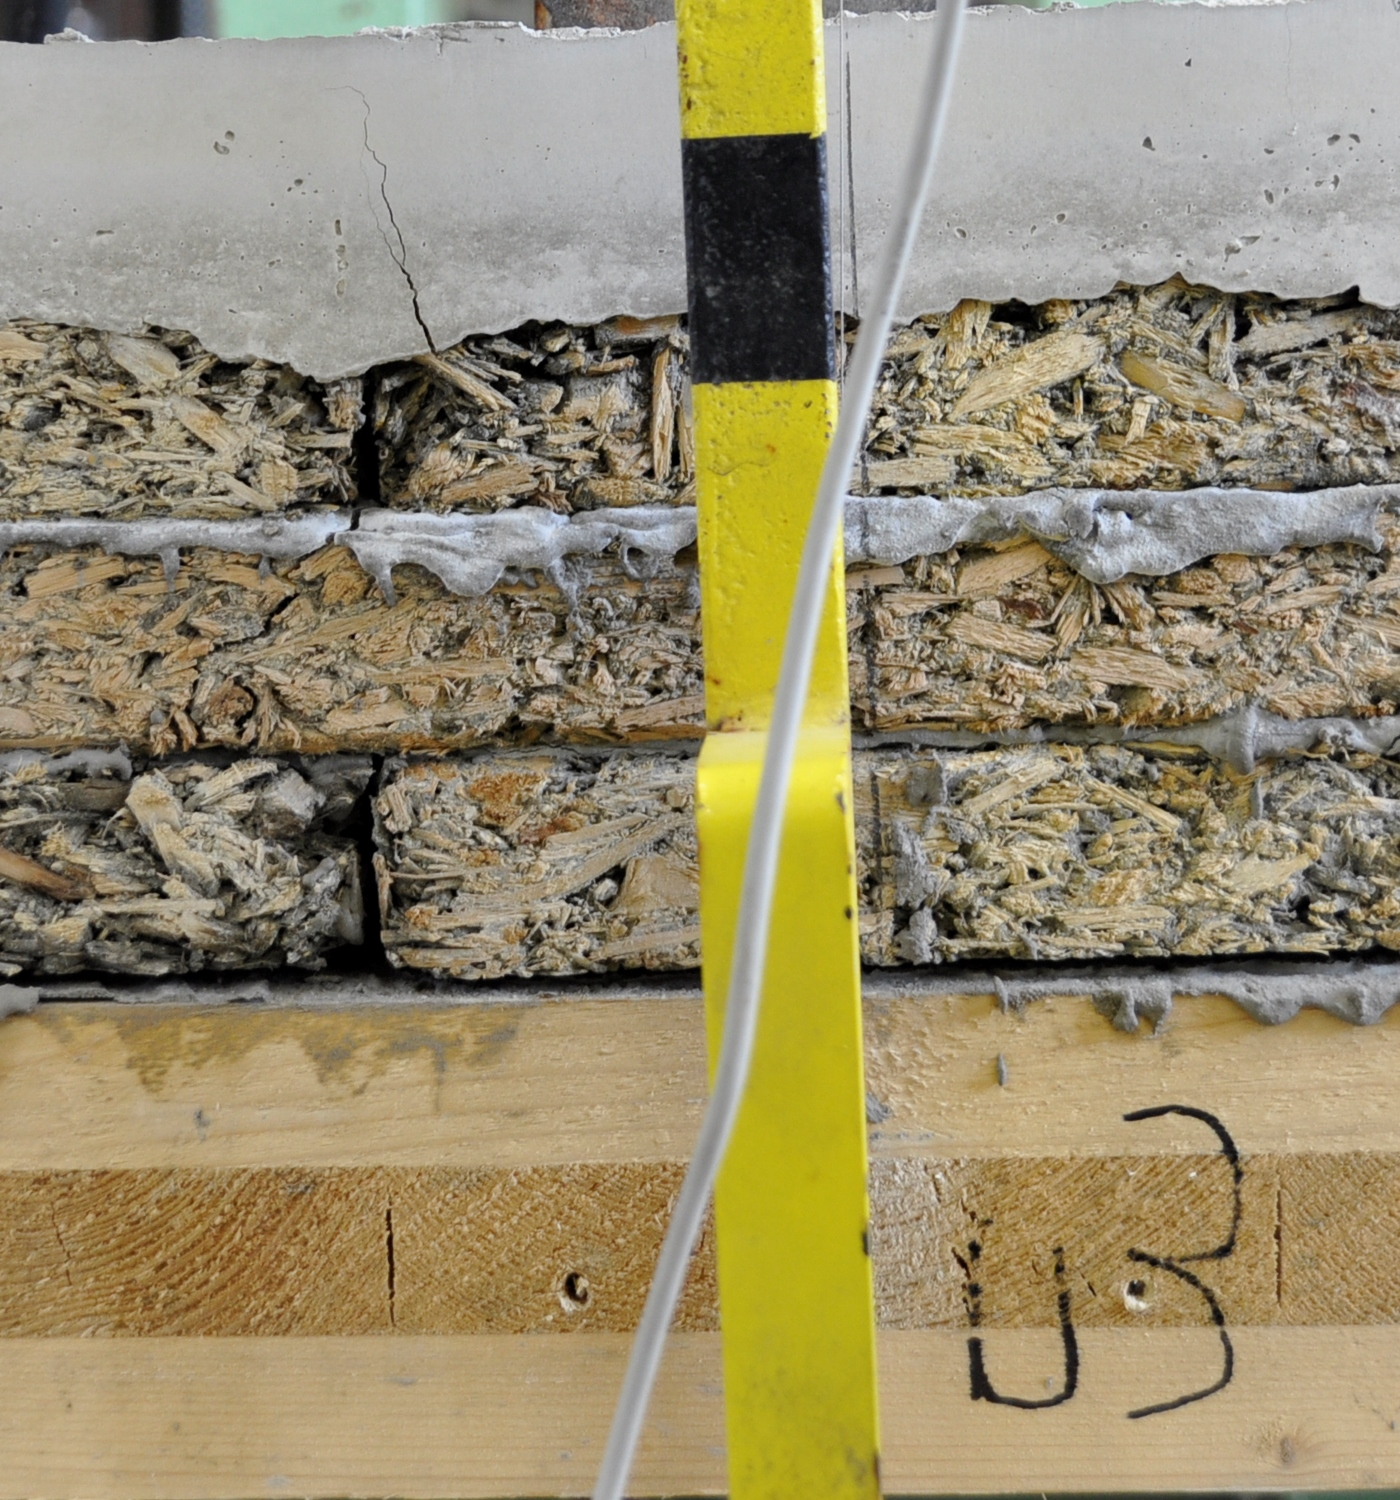
\includegraphics[width=7cm]{4versuch_schichtbruch.jpg}
	\caption{Risse in der Beton-und Veloxschicht}
	\label{4versuch_schichtbruch}
\end{minipage}
\end{figure}

In den Abblindungen \ref{4versuch_auflagerB} und \ref{4versuch_auflagerA} sind die Oberflächen abgebildet, im Bereich der beiden Auflager. Es sind Teilflächen zu erkennen, welche noch die Riffen der Zahnspachtel aufweisen und Teilflächen auf der gegenüber liegenden Seite, die keine Benetzung mit dem Kleber vorweisen. In diesen Bereich hat nie ein Verbund stattgefunden. Es liegt hier kein Versagen der Veloxschicht vor, ausschließlich von der Klebeschicht, da nur geringe Spuren des Klebers auf der Veloxplatte feststellt wurde. Es ist zu Vermuten, dass während des Aushärten des Klebers, sich die Veloxplatten gekrümmt haben. 



\begin{figure}[h]
\begin{minipage}[hbt]{7cm}	
	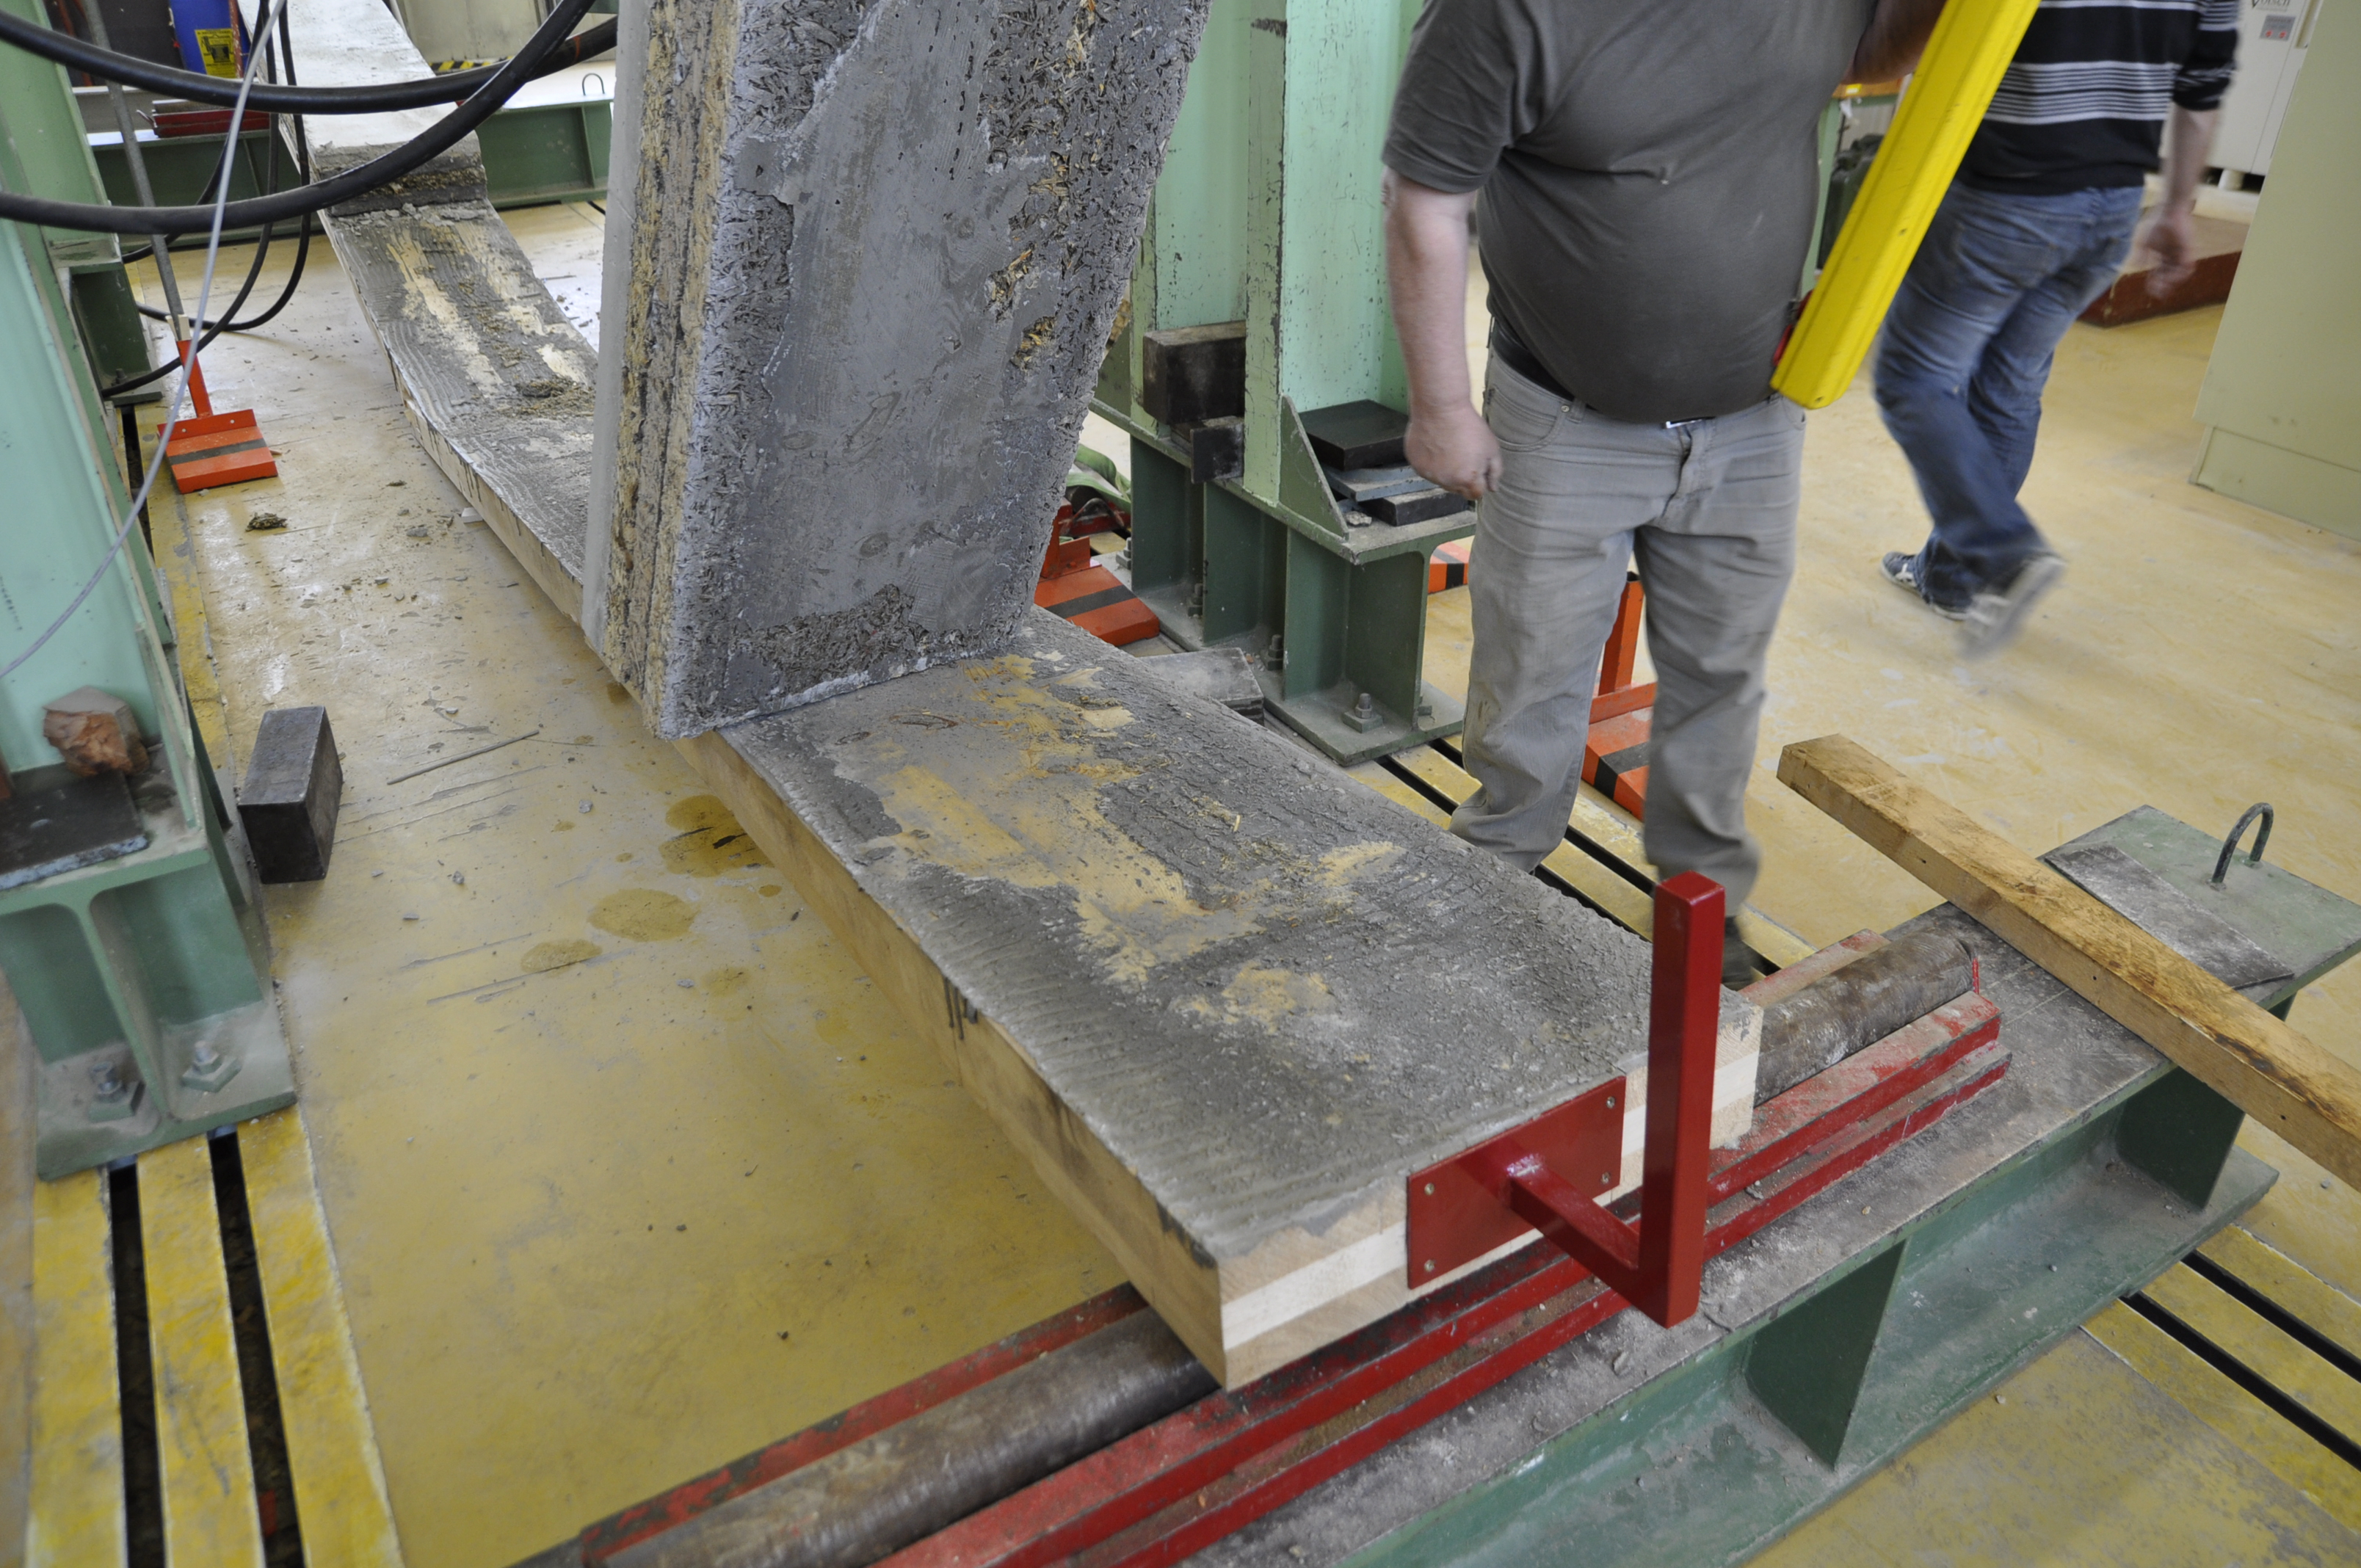
\includegraphics[width=7cm]{4versuch_auflagerB.jpg}
	\caption{Oberfläche der Klebefuge im Auflagerbereich B}
	\label{4versuch_auflagerB}
\end{minipage}
\hfill
\begin{minipage}[hbt]{7cm}
	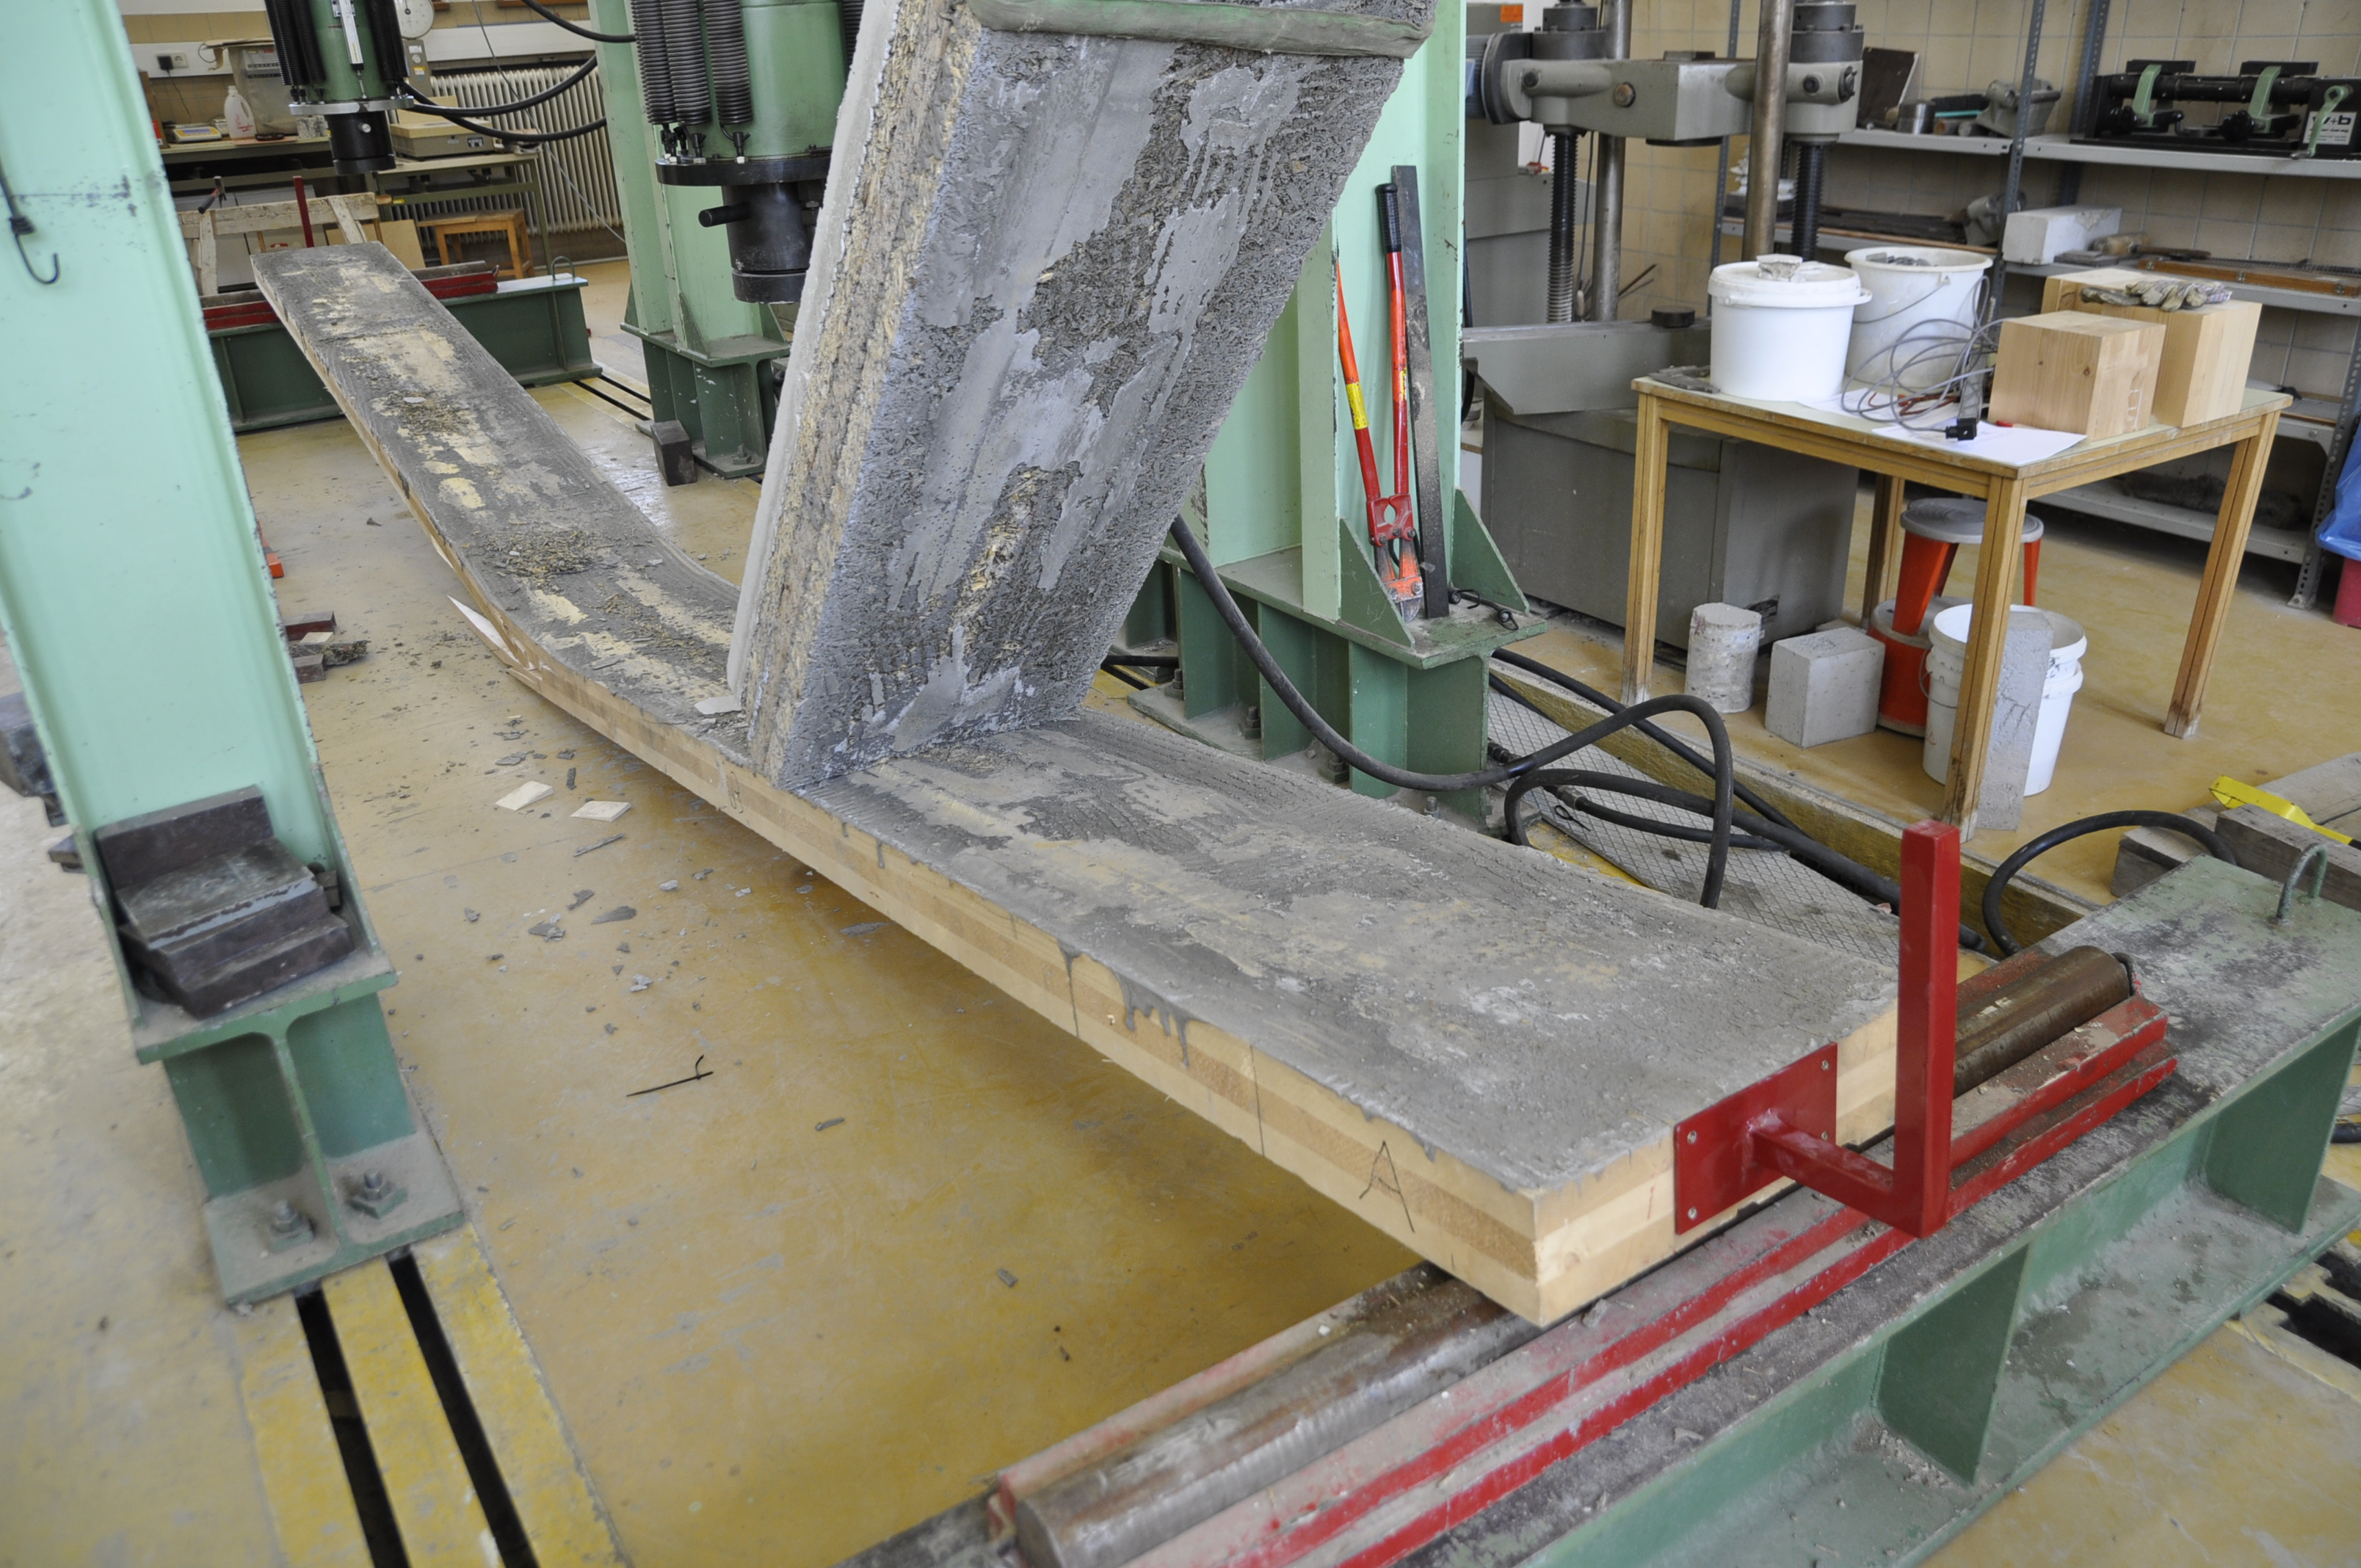
\includegraphics[width=7cm]{4versuch_auflagerA.jpg}
	\caption{Oberfläche der Klebefuge im Auflagerbereich A}
	\label{4versuch_auflagerA}
\end{minipage}
\end{figure}

\begin{figure}
	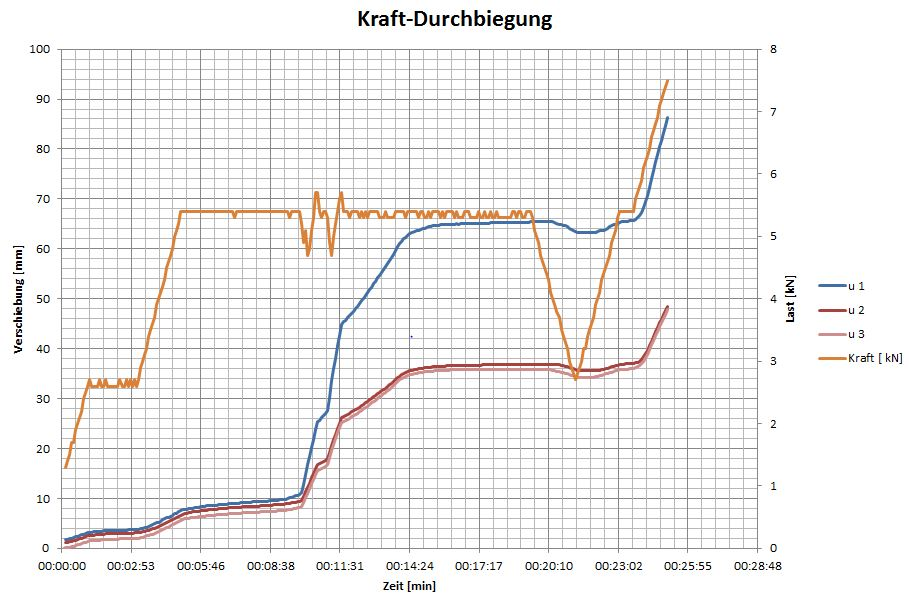
\includegraphics[scale=0.7]{4versuch_kraft_durchbiegung_zeit.jpg}
	\caption{4 Versuch: Kraft-Durchbiegung-Zeit}
	\label{4 Versuch: Kraft-Durchbiegung-Zeit}
\end{figure}


\begin{figure}	
	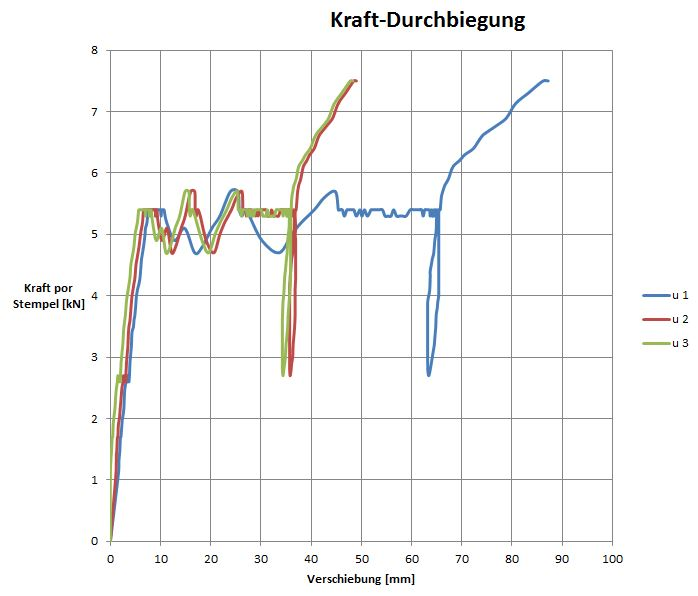
\includegraphics[scale=0.9]{4versuch_kraft_durchbiegung.jpg}
	\caption{4 Versuch: Kraft-Durchbiegung}
	\label{4 Versuch: Kraft-Durchbiegung}
\end{figure}



In der Abbildung \ref{4 Versuch: Kraft-Durchbiegung} und \ref{4 Versuch: Kraft-Durchbiegung-Zeit} sind die Arbeitslinie der Kraft Durchbiegung bzw. bezogen auf die Zeit dargestellt. In der Abbildung \ref{3 Versuch: Kraft-Durchbiegung-Zeit} ist der Kraftverlauf darstellt, der wie in Kapitel 4.7 beschrieben ist.  Da der Bauteil schon bei den unteren Laststufen (5,4 kN) ein ausgeprägtes Kriechverhalten aufwies, wurde die Laststufe länger gehalten. Auch in der Laststufe (2,7 kN) ist ein schon ein Kriechanteil ersichtlich. Die zacken in der Lastlinie sind dadurch gegeben, weil die Prüfmaschiene Lastgesteuert agiert. Bei Betrachtung der Verschiebungskennlinien, ist zu erkennen, dass sie eine fast idente Verschiebung vorweisen. Ab den Zeitpunkt(11::11:1), wächst die Verformung der Kennlinie u 1 stark an. Dies ist auf das Versagen der Veloxschicht zurückzuführen. Es sind in diesem Abschnitt auch zwei größere Sprünge in der Lastlinie aufgetreten. Die Verschiebungen u 2 und u 3 weisen auch Sprünge vor. Bei der Entlastung auf das Lastniveau von 2,7 kN, ist nur ein sehr geringer Rückgang der Verschiebungskennlinien ersichtlich, was auf eine nichtelastisches Verhalten des Bauteils hinweist. 
In der Abbildung\ref{4 Versuch: Kraft-Durchbiegung} sind die Verformung, unabhängig von der Zeit dargestellt. Es ist hier ein steiler Anstieg der Kennlinie ersichtlich. Bei der Laststufe 5,4 kN ist wieder ein sehr ausgeprägtes Kriechverhalten des Bauteil feststellbar. Bei der Absenkung der Last, auf 2,7 kN und anschließender Laststeigerung ist kein Rückgang der Verformungen erkennbar, war auf ein nichtelasttisches Verhalten des Bauteils hindeutet.


\begin{figure}
\begin{center}
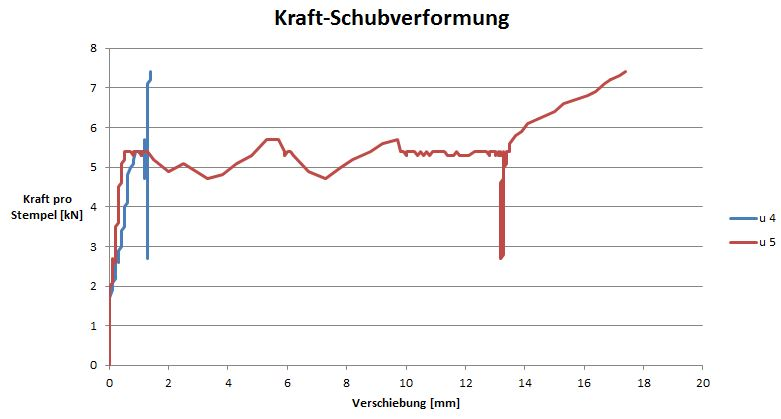
\includegraphics[scale =0.6]{4versuch_kraft_schubverformung.jpg}
\caption{4 Versuch: Kraft-Schubverformung}
\label{4_versuch_kraft_schubverschiebung}
\end{center}
\end{figure}



In der Abbildung \ref{4_versuch_kraft_schubverschiebung} die Arbeitslinie der Kraft Schubverformung dargestellt. Die Kennlinien sind bis zu dem Lastniveau von 5,4 kN fast ident. Die Sprünge der in der Kennlinie sind durch die geringe Auflösung der Messaufnehmer bedingt. Daher sind die Verschiebungen bis zur Last von 2 kN nicht dargestellt. Beim der konstanten Last von 5,4 kN ist in der Kennlinie u 5 die am Auflager A gemessen worden ist, gegenüber Kennlinie u 5 ein großer Verschiebungsanteil erkennbar. Die Verschiebung war auch beim Versuch visuell zu beobachten.  


\section{Vergleich}



\begin{figure}
\begin{center}
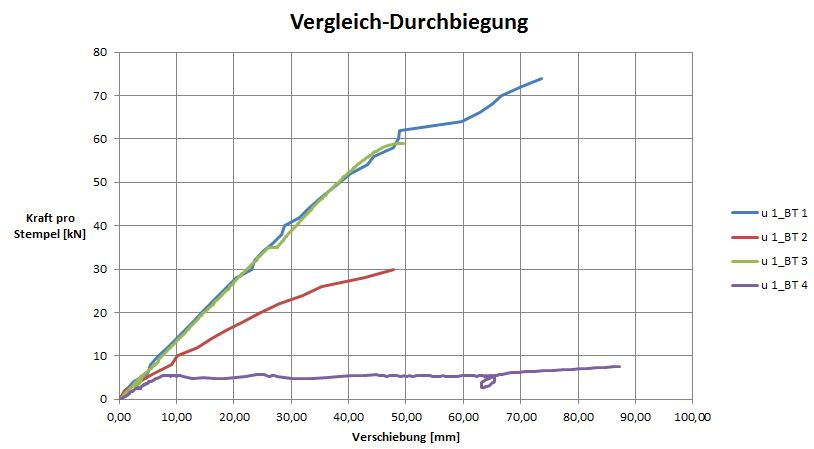
\includegraphics[scale =0.6]{vergleich-durchbiegung.jpg}
\caption{Vergleich der Verschiebungskennlinien in Bauteilmitte}
\label{vergleich-durchbiegung}
\end{center}
\end{figure}

In der Abbildung \ref{vergleich-durchbiegung} sind die Durchbiegungskennlinien in der Mitte des Bauteiles (u 1) angeführt.
Es fällt sofort auf, das die Arbeitslinien der Bauteile 1 und 3 eine sehr große Übereinstimmung aufweisen. Die Bauteile unterscheiden sich in der Anzahl der Schrauben und des unterschiedlichen Kleber. Man muss hier auf die Tabelle \ref{tab:Versuchsprogramm} verweisen, in der die Anzahl der Schrauben aufgelistet ist. Es scheint, dass der Anzahl der Schrauben in Bezug auf die Durchbiegung, nur einen geringen Einfluss hat. Der zweite Bauteil weist eine geringe Steigung auf, dass auf die Vorschädigung zurückzuführen ist. Durch die Verwendung des schlechteren Klebers und die Verminderung der Schraubenanzahl, kann der Abfall erklärt werden. Der vierte Bauteil hatte keine mechanischen Verbindungmittel in Verwendung, daher waren auch schon vor dem Versuch bzw. beim einbringen in die Prüfmaschine, Schädigungen entstanden. 
Es ist festzustellen, dass das Sandwich ohne mechanische Verbingungsmittel, eine zu geringe Steifigkeit aufweist. Jedoch kann die Anzahl, auf ein minimum gesetzt werden.


\begin{figure}
\begin{center}
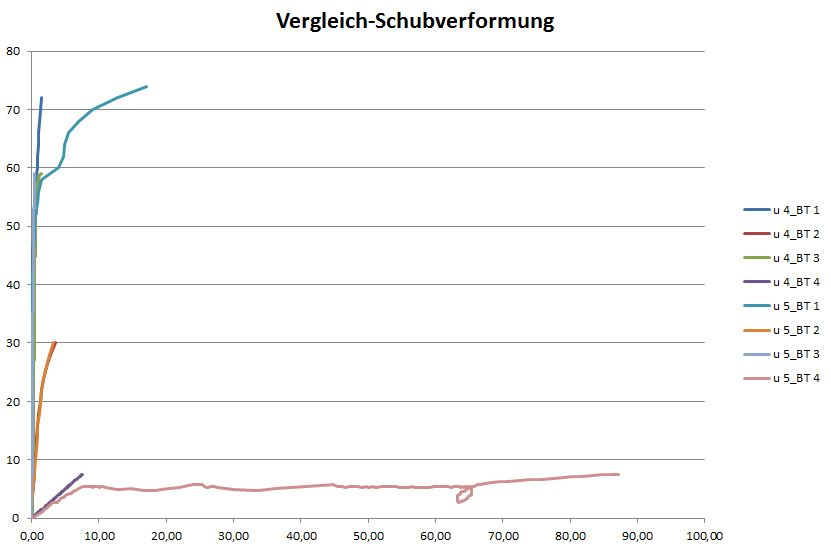
\includegraphics[scale =0.6]{vergleich-schubverformung.jpg}
\caption{Vergleich der Schubverformujngskennlinien}
\label{vergleich-schubverformung}
\end{center}
\end{figure}

Bei der Betrachtung der Schubverformungen, wie in der Abbildung \ref{vergleich-schubverformung} ersichtlich, liegen die Arbeitslininen des ersten und dritten Versuchs sehr nahe beisammen. Dieser Vergleich ist auch bei der Durchbiegungskennlinien zu sehen. Die Unterschiede sind im vorrigen Absatz schon erläutert worden. Es kann die Annahme getroffen werden, dass die Anzahl der Schrauben keinen linearen Einfluss aufweisen. Die Kennlinie des Bauteil 2 hat bis zu 20 kN die gleiche Steigung, jedoch krümmt sich die Linie, mit der Zunahme der Kraft. Der vierte Bauteil hat im Gegensatz zu den vorgehenden Versuchen eine sehr flache Kurve. Dies ist wiederum auf den Verzicht auf mechanische Verbindungsmittel zurück zu führen.




\end{document}













